%% LyX 2.0.8.1 created this file.  For more info, see http://www.lyx.org/.
%% Do not edit unless you really know what you are doing.
\documentclass[english,11pt]{scrartcl}
\usepackage[LGR,T1]{fontenc}
\usepackage[latin9]{inputenc}
\usepackage{listings}
\lstset{basicstyle={\ttfamily\small},
commentstyle={\color{comment}},
identifierstyle={\color{var}},
keywordstyle={\color{kw}},
language=Matlab,
stringstyle={\color{str}},
upquote=true}
\setlength{\parskip}{\medskipamount}
\setlength{\parindent}{0pt}
\usepackage{color}
\usepackage{babel}
\usepackage{array}
\usepackage{float}
\usepackage{textcomp}
\usepackage{amsthm}
\usepackage{amsmath}
\usepackage{amssymb}
\usepackage{graphicx}
\usepackage[unicode=true,pdfusetitle,
 bookmarks=true,bookmarksnumbered=false,bookmarksopen=false,
 breaklinks=false,pdfborder={0 0 0},backref=false,colorlinks=true]
 {hyperref}

\makeatletter

%%%%%%%%%%%%%%%%%%%%%%%%%%%%%% LyX specific LaTeX commands.
\DeclareRobustCommand{\greektext}{%
  \fontencoding{LGR}\selectfont\def\encodingdefault{LGR}}
\DeclareRobustCommand{\textgreek}[1]{\leavevmode{\greektext #1}}
\DeclareFontEncoding{LGR}{}{}
\DeclareTextSymbol{\~}{LGR}{126}
\newcommand{\lyxmathsym}[1]{\ifmmode\begingroup\def\b@ld{bold}
  \text{\ifx\math@version\b@ld\bfseries\fi#1}\endgroup\else#1\fi}

%% Because html converters don't know tabularnewline
\providecommand{\tabularnewline}{\\}

%%%%%%%%%%%%%%%%%%%%%%%%%%%%%% Textclass specific LaTeX commands.
\newcommand*{\Rinput}[1]{\mbox{\lstinline!#1!}}
\newcommand{\code}[1]{\texttt{#1}}

%%%%%%%%%%%%%%%%%%%%%%%%%%%%%% User specified LaTeX commands.
\usepackage[scaled=0.9]{helvet}
\usepackage[T1]{fontenc}
\usepackage[scaled=0.9]{beramono}

\usepackage{microtype}
\usepackage{mathpazo,textcomp}

\usepackage{fancyvrb}
\usepackage{color}
\definecolor{lightgray}{gray}{0.5}
\setlength{\parindent}{0pt}

\typearea{12}

\definecolor{darkblue}{cmyk}{1,0,0,0.8}
\definecolor{darkred}{cmyk}{0,1,0,0.7}
\definecolor{orange}{cmyk}{0,0.5,1,0}
\hypersetup{anchorcolor=black,
  citecolor=darkblue, filecolor=darkblue,
  menucolor=darkblue,pagecolor=darkblue,urlcolor=darkblue,linkcolor=darkblue}

\definecolor{var}{rgb}{0,0.25,0.25}
\definecolor{comment}{rgb}{0,0.5,0}
\definecolor{kw}{rgb}{0,0,0.5}
\definecolor{str}{rgb}{0.5,0,0}

\usepackage{upquote}

\newcommand{\blist}[1]{\mbox{\lstinline!#1!}}

\makeatother

\begin{document}

\title{Description of the extension ddebiftool\_nmfm}


\author{Maikel Bosschaert, Bram Wage and Yuri Kuznetsov}


\date{16 September 2015}
\maketitle
\begin{abstract}
This addendum describes the normal form extension\texttt{ }to DDE-BifTool,
a bifurcation analysis toolbox running in \texttt{Matlab}%
\footnote{\href{http://www.mathworks.com}{http://www.mathworks.com}%
} or \texttt{GNU Octave}%
\footnote{\href{http://www.gnu.org/software/octave}{http://www.gnu.org/software/octave}%
}. For systems of DDEs with constant delays this extension is able
to automatically detect and accurately locate fold and Hopf bifurcations
on steady-state branches, as well as generalized Hopf, double-Hopf,
fold-Hopf, Bogdanov-Takens and cusp bifurcations on Hopf and/or fold
branches. In addition, the critical normal from coefficients of the
bifurcations are computed. This will be illustrated with three different
example systems.
\end{abstract}
\tableofcontents{}


\section{Overview}

Users unfamiliar with DDE-BifTool should look at the demo in the folder
\texttt{minimal\_demo} (script \texttt{rundemo.m}). In Section \ref{sec:Example1}
a model of two interacting layers of neurons\textbf{ }will be used
to demonstrate the detection of and normal form coefficient computation
for Hopf, generalized Hopf, double-Hopf and fold-Hopf bifurcations.
In Section \ref{sec:Example2} a system exhibiting a Bogdanov-Takens
bifurcation is considered. Here, the sign of the critical normal form
coefficients is verified by looking at the stability of the cycles.
Lastly, in Section (\ref{sec:Example3}) a system with cusp and Bogdanov-Takens
is presented.

In version 3.1 of DDE-BifTool a normal form extension, written by
Bram Wage \cite{W14}, was supplied. Here we give a short list of
changes and additions that have been made:


\paragraph{1. }

The normal form extension is now able to detect, locate and compute
critical normal form coefficients in the following situations
\begin{itemize}
\item Hopf encountered along steady-state curves
\item Generalized Hopf, fold-Hopf and double-Hopf encountered along Hopf
curves
\item Fold encountered along steady-state curves
\item Cusp, Bogdanov-Takens and fold-Hopf encountered along Fold curves
\item Bogdanov-Takens encountered along Hopf curves
\end{itemize}
Previously only the first two items were supported. In other words,
all codimension-1 bifurcations typically encountered on steady-state
curves and codimension-2 bifurcations typically encountered on either
fold or Hopf curves are now implemented.


\paragraph{2. }

The function to detect bifurcations, \blist{br\_bifdet.m}, has been
completely rewritten and is now supporting 
\begin{itemize}
\item Detection of multiple bifurcations occurring in the same interval
on a bifurcation curve
\item Plotting of the test function used to detect the bifurcation
\item Realtime monitoring of the eigenvalues
\end{itemize}

\paragraph{3.}

The code to locate codimension-2 bifurcation has been separated into
a new function \blist{locate\_codim2}, instead of being repeated
for every bifurcation detected. In the previous version, the middle
point selected in the bisection method was not correct in the generalized
Hopf and fold-Hopf cases; this has been fixed.


\paragraph{4.}

The test functions indicating Hopf encountered along steady-state
curves and fold-Hopf encountered along Hopf curves have been changed.
Now the test function for Hopf uses the same function as for the double-Hopf
bifurcation. See (\ref{eq:testfunction_FH_H}) for the new test function
used to detect fold-Hopf. 


\paragraph{5.}

Abbreviations used for codimension-2 bifurcation have been changed
to mimic those being used in MatCont%
\footnote{\href{https://sourceforge.net/projects/matcont/}{https://sourceforge.net/projects/matcont/}%
}.


\section{Delay differential equations}

Consider a system of delay differential equations with constant delays
(DDE),

\begin{equation}
\dot{x}(t)=f(x(t-\tau_{0}),x(t-\tau_{1}),\ldots,x(t-\tau_{m}),\alpha),\label{eq:discrete_dde}
\end{equation}
where $x(t)\in\mathbb{R}^{n}$, $f:\mathbb{R}^{n(m+1)}\times\mathbb{R}^{p}\rightarrow\mathbb{R}^{n}$
is a smooth function depending on a number of parameters $\alpha\in\mathbb{R}^{p}$,
and delays $\tau_{i}$, $i=0,\ldots,m$, ordered such that $0=\tau_{0}\leq\tau_{1}\leq\dots\leq\tau_{m}$
. Assume that 
\[
f(x^{*},\ldots,x^{*},\alpha_{0})=0.
\]
Then $x^{*}$ is a stationary point at $\alpha=\alpha_{0}$ and to
which we can associate the linearized problem 
\begin{equation}
\dot{y}(t)=A_{0}(x^{*},\alpha_{0})y(t)+\sum_{i=1}^{m}A_{i}(x^{*},\alpha_{0})y(t-\tau_{i}),\label{eq:linearized_problem}
\end{equation}
 where, using $f\equiv f(x^{0},x^{1},\ldots,x^{m},\alpha)$, 
\[
A_{i}(x^{*},\alpha_{0})=\frac{\partial f}{\partial x^{i}}(x^{*}(0),x^{*}(-\tau_{1}),\ldots,x^{*}(-\tau_{m}),\alpha_{0}),\ i=0,\ldots,m
\]
Define the $n\times n$-dimensional matrix $\Delta$ as 
\begin{equation}
\Delta(x^{*},\alpha_{0},\lambda)=\lambda I-A_{0}(x^{*},\alpha_{0})-\sum_{i=1}^{m}A_{i}(x^{*},\alpha_{0})e^{-\lambda\tau_{i}}.\label{eq:characteristic_matrix}
\end{equation}
 Then the characteristic equation reads 
\begin{equation}
\det(\Delta(x^{*},\alpha_{0},\lambda))=0.\label{eq:characteristic_equation}
\end{equation}
We refer to roots of the characteristic equation as eigenvalues. The
stability of a generic stationary point is determined by its eigenvalues,
see \cite{diekmann2012delay}. In particular, when eigenvalues cross
the imaginary axis in the complex plane, bifurcations occur. To simplify
notation we write $\Delta(\lambda)$ for $\Delta(x^{*},\alpha_{0},\lambda)$
when no confusion arises.


\section{Detecting and locating codimension-1 bifurcation}


\subsection{Test functions\label{sub:Test-functions_stst}}

A function along the considered branch that has a regular zero at
a bifurcation is called a test function. Below we will simply list
functions used for detecting certain bifurcations without proving
their regularity.

There is a real number $\xi$ such that all zeros of $\mbox{det}\Delta(\lambda)$
are in the left half plane $\left\{ z\in\mathbb{C}\vert\mbox{Re}z<\xi\right\} $.
If in the linearized problem (\ref{eq:linearized_problem}) not all
$A_{i}$ vanish simultaneously, then $\mbox{det}\Delta(\lambda)$
has infinitely many roots such that there is only a finite number
of solutions in any vertical strip in the complex plane. For detecting
bifurcations depending on the eigenvalues we can therefore look at
a vertical strip containing zero. Care must be taken when constructing
test functions based on these eigenvalues in a chosen vertical strip.
Indeed, the number of eigenvalues in the vertical strip may vary as
parameters change. For this reason we prefer to use detection methods
relaying on the Jordan chains of the characteristic matrix $\Delta(\lambda)$
whenever possible.

After a test function indicates a bifurcation by changing its sign,
we need to locate the bifurcation point accurately in order to calculate
the critical normal form coefficients. As we will see below, we use
the bisection method or apply Newton on a specially constructed defining
system to achieve this.

When continuing a steady-state of a DDE, we generally expect to encounter
codimension-1 bifurcations, that is fold or Hopf bifurcations. We
therefore start by defining test functions for these two bifurcations.


\subsection{Fold $(\lambda_{1}=0)$}

At a fold point the characteristic equation $\mbox{det}\Delta(\lambda)=0$
has a simple eigenvalue $\lambda_{1}=0$ and no other eigenvalues
on the imaginary axis. A test function to detect this bifurcation
is given by
\[
\psi_{f}=\mbox{det}\Delta(0).
\]


To locate the fold point, the defining system
\begin{equation}
S_{f}(x,q,\alpha)=\begin{pmatrix}f(x,\dots,x,\alpha)\\
\Delta(x,\alpha,0)q\\
c^{T}q-1
\end{pmatrix}=0\label{eq:DS_hopf_at_BT-1}
\end{equation}
is used. Here $c^{T}q-1$ presents a suitable normalization of $q\in\mathbb{R}^{n}$.
The vector $c\in\mathbb{R}^{n}$ is chosen as $c=q^{(0)}/(q^{(0)^{T}}q^{(0)})$,
where $q^{(0)}$ is the initial value of $q$. Solving this system
by Newton's method gives $(x,q,\alpha)$, corresponding to the fold
point.


\subsection{Hopf $(\lambda_{1,2}=\pm i\omega_{0})$\label{sub:Hopf}}

At a Hopf point the characteristic equation $\det\Delta(\lambda)=0$
has a pair of purely complex conjugate eigenvalues $\lambda=\pm i\omega$,
with $\omega>0$, and no other eigenvalues on the imaginary axis.
For a test function we look at the sign of the smallest real part
of the complex eigenvalue pairs. For this the following function has
been constructed
\begin{lstlisting}[basicstyle={\footnotesize},language=Matlab]
function [smallest_real_part, stability,selectedroot] = nmfm_smrp(...     
funcs,point, stmethod,varargin) 
%% Compute smallest real part of imaginary pairs or of real eigenvalues 
% 
% * rmomega (logical): remove known imaginary roots 
% * threshold (function): threshold(abs(imag(roots)) selects roots to 
% consider 
% 
% $Id: nmfm_smrp.m 73 2014-12-31 10:47:51Z jan.sieber $ 
% 
%% default={'stabilityfield','l1','remove_omega',false, ...
%  'threshold',@(x)true(size(x))}; 
options=dde_set_options(default,varargin); 
if ~isfield(point, 'stability') || isempty(point.stability) || ...
		isempty(point.stability.l0)
	point.stability = p_stabil(funcs,point, stmethod); 
end

stability = point.stability; 
roots = stability.(options.stabilityfield);

%% Remove roots closest to known eigenvalue pair 
if options.remove_omega
   [dum,ix]=sort(abs(roots - 1i*point.omega)); %#ok<ASGLU>
   roots(ix(1))=[];
   [dum,ix]=sort(abs(roots + 1i*point.omega)); %#ok<ASGLU>
   roots(ix(1))=[];
end

selectedroots = roots(options.threshold(abs(imag(roots)))); 
if isempty(selectedroots)
   smallest_real_part = 0;
   return 
end 
%% Assume all imaginary eigenvalues come in pairs
realparts = real(selectedroots); 
[dum, rpind] = sort(abs(realparts)); %#ok<ASGLU> 
smallest_real_part = realparts(rpind(1)); 
selectedroot=selectedroots(rpind(1)); 
end
\end{lstlisting}
The value of the test function $\psi_{H}$ at the $i$th point on
the steady-state branch is then given by
\[
\psi_{H}(i)=\text{nmfm\_smrp(funcs,p,stmethod,'remove\_omega',false,'threshold',isimag)}.
\]
Here \blist{isimag=@(x)x>imagthresh} is an anonymous function that
selects all eigenvalues that have imaginary parts greater than \blist{imagthresh}.
If there are no complex eigenvalues according to this rule the function
returns the zero value. Since a sign change is monitored by
\[
|\text{sign}(\phi_{H}(i))+\text{sign}(\phi_{H}(i-1))|,
\]
we have to exclude the case $\phi_{H}(i)=0$ while detecting.

When a bifurcation is detected we locate the Hopf point using the
defining system
\begin{equation}
S_{H}(x,q,\alpha,\omega)=\begin{pmatrix}f(x,\dots,x,\alpha)\\
\Delta(x,\alpha,i\omega)q\\
c^{H}q-1
\end{pmatrix}=0.\label{eq:DS_hopf_at_BT}
\end{equation}
Here $c^{H}q-1$ presents a suitable normalization of $q\in\mathbb{C}^{n}$.
The vector $c\in\mathbb{\mathbb{C}}^{n}$ is chosen as $c=q^{(0)}/(q^{(0)^{H}}q^{(0)})$,
where $q^{(0)}$ is the initial value of $q$. Solving this system
by Newton's method gives $(x,q,\alpha,\omega)$, corresponding to
the Hopf point.


\section{Detecting and locating codimension-2 bifurcations\label{sec:Detecting-and-locating}}

Due to the existence of a finite-dimensional smooth center manifold
for Delay Differential Equations it is possible to `lift' the normal
form theory for Ordinary Differential Equations (ODEs) to DDEs. The
ODE on the center manifold can be transformed into a normal form by
smooth invertible substitutions of the coordinates. The critical normal
form coefficients can be calculated with different methods. In \cite{Janssens:Thesis}
the theory of sun-star calculus was combined with the approach used
in \cite{Kuznetsov:Elements:2004} for calculating critical normal
form for ODEs. We refer to \cite{Janssens:Thesis} for the derivation
of the critical normal form coefficients. Here we will simply list
the critical normal forms on the center manifold and demonstrate how
to compute their coefficients. Readers familiar with normal forms
for ODEs will notice the similarity. The major difference is seen
in the vectors used in the critical coefficients. In ODEs eigenvectors
and generalized eigenvectors of the Jacobian of the system appear
in the coefficients. In DDEs the vectors used in the coefficients
are obtained from the Jordan chains of the characteristic matrix (\ref{eq:characteristic_matrix}).

When investigating two-parameter problems, one usually encounters
higher-order degeneracies along codimension-1 bifurcation curves.
Some of these degeneracies are determined by the characteristic matrix,
while others can only be detected using the non-linear terms of (\ref{eq:discrete_dde}).
For this reason we start the section with the critical normal forms
for codimension-1 equilibrium bifurcations, namely the fold and Hopf.


\subsection{Normal forms for codimension-1 bifurcations}

Consider the steady-state $x^{*}$ of (\ref{eq:discrete_dde}) at
$\alpha=\alpha_{0}$. By a shift of coordinates and parameters it
can always be arranged that $x^{*}=0$ and $\alpha_{0}=0$. Since
we are only calculating the critical normal form coefficients, we
drop the parameter and write $f(x^{0},x^{1},\ldots,x^{m})$. To simplify
notation we write $f^{0}$ for $f(x^{*},x^{*},\ldots,x^{*})$. Expanding
$f$ in $X=\left(x^{0},x^{1},\ldots,x^{m}\right)\in\mathbb{R}^{n}\times\mathbb{R}^{m+1}$
around $(x^{*},x^{*},\ldots,x^{*})$ yields 
\begin{align}
\begin{aligned}f(X) & =\left(Df^{0}\right)X+\frac{1}{2}\left(D^{2}f^{0}\right)(X,X)+\frac{1}{3!}\left(D^{3}f^{0}\right)(X,X,X)\\
 & \qquad+\frac{1}{4!}\left(D^{4}f^{0}\right)(X,X,X,X)+\frac{1}{5!}\left(D^{5}f^{0}\right)(X,X,X,X,X)+\mathcal{O}(X^{6}),
\end{aligned}
\label{eq:multilinear-form}
\end{align}
where
\begin{align*}
Df_{i}^{0}(q) & =\sum_{j=0}^{m}\frac{\partial f_{i}^{0}}{\partial x^{j}}q^{j}=\sum_{k=1}^{n}\sum_{j=0}^{m}\frac{\partial f_{i}^{0}}{\partial x_{k}^{j}}q_{i}^{j},\\
D^{2}f_{i}^{0}(q,p) & =\sum_{j_{1},j_{2}=0}^{m}\frac{\partial f_{i}^{0}}{\partial x^{j_{1}}\partial x^{j_{2}}}q^{j_{1}}p^{j_{2}}\\
 & =\sum_{k_{1},k_{2}=1}^{n}\sum_{j_{1},j_{2}=0}^{m}\frac{\partial f_{i}^{0}}{\partial x_{k_{1}}^{j_{1}}\partial x_{k_{2}}^{j_{2}}}q_{i_{1}}^{j_{1}}p_{i_{2}}^{j_{2}},
\end{align*}
for $1\leq i\leq n$. The multilinear forms $D^{3}f^{0}(p,q,z),\, D^{4}f^{0}(p,q,z,v)$
and $D^{5}f^{0}(p,q,z,v,w)$ can be expressed similarly.


\subsubsection{Fold $(\lambda_{1}=0,\, b\protect\neq0)$}

If the steady-state $x^{*}\equiv0$ of (\ref{eq:discrete_dde}) has
a fold bifurcation at the parameter value $\alpha_{0}=0$, then the
characteristic equation $\det\Delta(\lambda)=0$ has a simple zero
$\lambda_{1}=0$. Then there exist vectors $q,p\in\mathbb{R}^{n}$
such that
\[
\Delta(0)q=0,\qquad p^{T}\Delta(0)=0.
\]
These can be normalized to satisfy 
\[
p^{T}\Delta'(0)q=1
\]
Here $\Delta'$ denotes the derivative of the characteristic equation
(\ref{eq:characteristic_equation}) with respect to $\lambda.$ The
restriction of (\ref{eq:discrete_dde}) to the one-dimensional center
manifold $W^{c}$ can be transformed to the form 
\begin{equation}
\dot{w}=bw^{2}+\mathcal{O}\left(|w|^{3}\right)\qquad w\in\mathbb{R},\label{eq:fold_nf}
\end{equation}
where the critical normal form coefficient is given by
\begin{equation}
b=\frac{1}{2}p^{T}D^{2}f^{0}(\Phi,\Phi),\label{eq:normal_form_fold_coef}
\end{equation}
with 
\begin{equation}
\Phi=(q,q,\dots,q)\in\mathbb{R}^{n}\times\mathbb{R}^{m+1}.\label{eq:PHI_fold}
\end{equation}
When a fold point is detected and located, the critical normal form
coefficient $b$ is reported in the Matlab console.


\subsubsection{Hopf $(\lambda_{1,2}=\pm i\omega_{0},\,\ell_{1}\protect\neq0)$}

If the steady-state $x^{*}\equiv0$ of (\ref{eq:discrete_dde}) has
a Hopf bifurcation at the parameter value $\alpha_{0}=0$, then the
characteristic equation $\det\Delta(\lambda)=0$ has a pair of purely
imaginary eigenvalues $\lambda_{1,2}=\pm i\omega_{0}$, with $\omega_{0}>0$,
and no other eigenvalues on the imaginary axis. Let $q,p\in\mathbb{R}^{n}$
such that
\[
\Delta(i\omega_{0})q=0,\qquad p^{T}\Delta(i\omega_{0})=0.
\]
These can be normalized to satisfy
\[
p^{T}\Delta'(i\omega_{0})q=1.
\]
The restriction of (\ref{eq:discrete_dde}) to the two-dimensional
center manifold $W^{c}$ can be transformed into the form
\[
\dot{z}=i\omega_{0}z+c_{1}z^{2}\bar{z}+\mathcal{O}(|z|^{4})\qquad z\in\mathbb{C}.
\]
The critical normal form coefficient in this expression is $c_{1}$.
The first Lyapunov coefficient is given by 
\begin{equation}
\ell_{1}=\frac{1}{\omega_{0}}\mbox{Re\,}c_{1},\label{eq:first_lyapunov_coeff}
\end{equation}
where 
\begin{align*}
c_{1} & =\frac{1}{2}p^{T}\Big[D^{2}f^{0}\left(\bar{\Phi},H_{20}\right)+2D^{2}f^{0}\left(\Phi,H_{11}\right)+D^{3}f^{0}(\Phi,\Phi,\overline{\Phi})\Big],
\end{align*}
with $\Phi$, $H_{20}$ and $H_{11}$ computed as follows. Let
\begin{align}
h_{20}(\vartheta) & =e^{2i\omega_{0}\vartheta}\Delta(\phi,\alpha_{0},2i\omega_{0})^{-1}D^{2}f^{0}(\Phi,\Phi),\nonumber \\
h_{11}(\vartheta) & =\Delta(\phi,\alpha_{0},0)^{-1}D^{2}f^{0}(\Phi,\overline{\Phi}),\label{eq:hopf_h11}\\
\phi(\vartheta) & =e^{i\omega_{0}\vartheta}q,\nonumber 
\end{align}
then 
\begin{align}
\Phi & =\left(\phi(0),\phi(-\tau_{1}),\dots,\phi(-\tau_{m})\right),\label{eq:PHI_Hopf}\\
H_{20} & =\left(h_{20}(0),h_{20}(-\tau_{1}),\dots,h_{20}(-\tau_{m})\right),\nonumber \\
H_{11} & =\left(h_{11}(0),h_{11}(-\tau_{1}),\dots,h_{11}(-\tau_{m})\right).\nonumber 
\end{align}
When a Hopf point is detected and located, the critical normal form
coefficient $\ell_{1}$ is reported in the Matlab console.


\subsection{Codimension-2 points on a fold curve $(\lambda_{1}=0)$\label{sub:test_functions_fold}}

While continuing a fold branch, the following codim-2 points can be
encountered:
\begin{enumerate}
\item An additional real eigenvalue $\lambda_{2}$ meets the imaginary axis,
with their geometric multiplicity remaining one, while the center
manifold $W^{c}$ becomes two-dimensional:
\[
\lambda_{1,2}=0.
\]
These are the conditions for a Bogdanov-Takens bifurcation. A test
function to detect this bifurcation is given by
\[
\psi_{BT}^{f}=p^{T}\Delta'(0)q.
\]
Here the vectors $p,q$ are calculated using the function \blist{eig}
from \texttt{Matlab}. Depending on the system being investigated,
this function does not always pass zero when a Bogdanov-Takens bifurcation
takes place on a Fold curve. For example the system in Section (\ref{sec:Example3})
exhibits this behavior, see Figure \ref{fig:fold_br_testfunctions}.
Therefore we also monitor the derivative of $\psi_{BT}^{f}$ with
respect to the parameters. We note that at a Bogdanov-Takens point
the normalization for the calculation of the critical normal form
coefficient $b$ of a fold point cannot be achieved anymore. This
we also see in Figure \ref{fig:fold_br_testfunctions}.
\item Two extra non-real eigenvalues $\lambda_{2,3}$ meet the imaginary
axis, and $W^{c}$ becomes three-dimensional:
\[
\lambda_{1}=0,\qquad\lambda_{2,3}=\pm i\omega_{0},
\]
for $\omega_{0}>0$. These conditions correspond to the fold-Hopf
bifurcation, also known as the Gavrilov-Guckenheimer bifurcation.
The test function is the same as the test function for a Hopf bifurcation
on a steady-sate branch, see Section (\ref{sub:Hopf})
\item The eigenvalue $\lambda_{1}=0$ remains simple and the only one on
the imaginary axis (dim $W^{c}=1$), but the normal form coefficient
$a$ in equation (\ref{eq:fold_nf}) vanishes
\[
\lambda_{1}=0,\, a=0.
\]
These are the conditions for a cusp bifurcation. The coefficient $b$
given in (\ref{eq:normal_form_fold_coef}) can be used as a test function
to detect this bifurcation:
\[
\psi_{CP}^{f}=b,
\]
where $b$ is given by (\ref{eq:normal_form_fold_coef}).
\end{enumerate}

\subsection{Codimension-2 points on a Hopf curve $(\lambda_{1,2}=\pm i\omega_{0})$\label{sub:test_functions_Hopf}}

While continuing a Hopf branch, the following codim-2 points can be
encountered:
\begin{enumerate}
\item An additional eigenvalue $\lambda_{3}=0$ meets the imaginary axis
and $W^{c}$ becomes three-dimensional:
\[
\lambda_{1,2}=\pm i\omega_{0},\qquad\lambda_{3}=0.
\]
As seen before these are the conditions for a fold-Hopf bifurcation.
For detection we can use the test function for a fold 
\begin{equation}
\psi_{FH}^{H}=\det\left(\Delta(0)\right).\label{eq:testfunction_FH_H}
\end{equation}

\item A Bogdanov-Takens bifurcation occurs when the two purely imaginary
eigenvalues $\lambda_{1}$ and $\lambda_{2}$ collide. We use 
\[
\psi_{BT}^{H}=\omega_{0}
\]
as a test function.
\item An additional pair of non-real eigenvalues $\lambda_{3,4}=\pm i\omega_{1}$,
meet the imaginary axis and $W^{c}$ becomes four-dimensional:
\[
\lambda_{1,2}=\pm i\omega_{0},\qquad\lambda_{3,4}=\pm i\omega_{1}.
\]
These conditions indicate a double-Hopf bifurcation. The value of
the test function for a double-Hopf bifurcation for the $i$th point
on a Hopf branch is given by
\[
\psi_{H}(i)=\text{nmfm\_mrp(funcs,p,stmethod,'remove\_omega',true,'threshold',isimag)}.
\]

\item As in the fold case, where $\lambda_{1}=0$ remains a simple zero
and the bifurcation is determined by a critical normal form coefficient,
there is also a bifurcation in the Hopf case where the dimension $W^{c}$
remains the same. When the first Lyapunov coefficient $\ell_{1}$
from (\ref{eq:first_lyapunov_coeff}) vanishes we have a generalized
Hopf bifurcation. The test function for a generalized Hopf point is
\[
\psi_{GH}=\ell_{1}.
\]

\end{enumerate}

\section{Implementation in DDE-BifTool}

\begin{table}
\begin{centering}
\begin{tabular}{|l|l|>{\raggedright}p{7cm}|}
\hline 
\textbf{Branch} & \textbf{Bifurcation} & \textbf{Test function}\tabularnewline
\hline 
\hline 
steady-state & fold & $\det\Delta(0)$\tabularnewline
\cline{2-3} 
 & Hopf & smallest real part of the complex eigenvalue pairs\tabularnewline
\hline 
fold & cusp & critical normal form coefficient $a$\tabularnewline
\cline{2-3} 
 & Bogdanov-Takens & $\psi_{BT}^{f}=p{}_{1}^{T}\Delta'(0)p_{0}$ or the derivative of $\psi_{BT}^{f}$\tabularnewline
\cline{2-3} 
 & fold-Hopf & smallest real part of the complex eigenvalue pairs\tabularnewline
\hline 
Hopf & Bogdanov-Takens & $\omega_{0}$\tabularnewline
\cline{2-3} 
 & fold-Hopf & $\det\Delta(0)$\tabularnewline
\cline{2-3} 
 & double-Hopf & smallest real part of the complex eigenvalue pairs\tabularnewline
\cline{2-3} 
 & generalized Hopf & first Lyapunov coefficient $\ell_{1}$\tabularnewline
\hline 
\end{tabular}
\par\end{centering}

\caption{An overview of bifurcations and monitored test functions.\label{tab:List-of-bifurcations}}
\end{table}


The call to the bifurcation routine is as follows:

\begin{lstlisting}[basicstyle={\footnotesize},language=Matlab]
[newbranch, success] = br_bifdet(branch)
\end{lstlisting}


Here, \blist{branch} is either a steady-state branch, fold branch
or Hopf branch, for which the stability has been calculated with \blist{br\_stabl}.
The \blist{newbranch} is a copy of \blist{branch}, but with possible
bifurcation points added. If bifurcation points are added \blist{success}
is set to 1, otherwise 0 will be returned. The function \blist{br\_bifdet}
will calculate the test function from Section (\ref{sub:Test-functions_stst}),
(\ref{sub:test_functions_fold}) or (\ref{sub:test_functions_Hopf}),
depending on type of branch, for every point on the branch. In Table
\ref{tab:List-of-bifurcations} these test functions are summarized.
If a sign change occurs the point is located. For fold and Hopf points
the function \blist{p\_correct}, from the default package, is used.
For codim-2 bifurcations the auxiliary function \blist{locate\_codim2}
has been written. After a bifurcation point is located successfully
the normal form coefficients are computed and stored in the \blist{nmfm}
structure of the corrected point. Lastly the function \blist{add\_to\_branch}
is called to add the corrected bifurcation point to the \blist{newbranch}.
In this function is checked if the distance between the bifurcation
point and the line connecting the last and second to last points on
the branch is no more than 25\% of the length of this line. If this
condition is satisfied the corrected bifurcation point is inserted
into \blist{newbranch}.


\subsection{Fields structure of \protect\blist{method.bifurcation}}

Fields of the structure \blist{method.bifurcation} , which is a substructure
of a branch structure.
\begin{itemize}
\item \blist{correction\_tolerance}: Custom value for \blist{method.point.minimal\_accuracy}
during \\
codimension-1 bifurcations correction. The default value is $10^{-7}$.
\item \blist{radial\_tolerance\_factor}: The maximum distance to the branch
the bifurcation point may have, relative to the distance between the
last two points. The default value is $0.25$.
\item \blist{secant\_iterations}: The maximum number of iterations for
the bisection method used to correct codimension-2 points. The default
value is 30.
\item \blist{secant\_tolerance}: The minimal accuracy for the bisection
method. The default value is $10^{-9}$.
\item \blist{plot\_testfunctions}: When set to 1 the test functions are
plotted. The default value is $0$.
\item \blist{monitor\_eigenvalues}: When set to 1 the eigenvalues of the
$i$th point on the branch are plotted. The default value is $0$.
\item \blist{pause\_on\_bifurcation}: When set to 1 the script will pause
when a bifurcation is detected and corrected. By pressing any key
the script will continue. The default value is $0$.
\item \blist{monitor\_eigenvalues\_time}: The time in seconds to pause
after plotting the eigenvalues of the $i$th point on the branch.
The default value is $0.1$.
\item \blist{imagthreshold}: Threshold for treating a number as complex
used in the function\\
 \blist{nmfm\_smrp}, see subsection \ref{sub:Hopf}. The default
value is set to $10^{-9}$. We note that setting this parameter to
zero didn't seem to affect the examples used in this manual.
\end{itemize}

\subsection{Locating codim-2 bifurcations, except Bogdanov-Takens}

If a codimension-2 bifurcation is detected, we want to locate the
bifurcation point. This is done with the bisection method:
\begin{enumerate}
\item Start with one point at which a test function is negative and one
point at which the test function is positive 
\item Construct the point halfway between the positive and the negative
point
\item Correct this point
\item Compute the test function at this point 
\item If the test function is negative, make this point the new negative
point; otherwise, the new positive point
\item Repeat until the absolute value of the test function is smaller than
some predefined tolerance
\end{enumerate}

\subsection{Locating Bogdanov-Takens}

\noindent For a Bogdanov-Takens bifurcation the defining system
\[
S(x,v,w,\alpha)=\begin{pmatrix}f(x,x,\dots,x,\alpha)\\
\Delta(x,\alpha,0)v\\
\Delta'(x,\alpha,0)v+\Delta(x,\alpha,0)w\\
(v,v)-1\\
(w,v)
\end{pmatrix}
\]
is used.


\subsection{Flagging bifurcation points}

When one has a branch of steady-states on which a Hopf bifurcation
occurs, one typically wants to plot the branch as a line and give
the Hopf point a special marker (e.g. a big dot). Ideally, one simply
passes an entire branch to a plot routine, along with an instruction
how to display the various bifurcations occurring along a branch.

Within the architecture of Matlab, this task provided a challenge.
As DDE-BifTool branches are stored as simple arrays of point-structures,
it was not possible to have a branch of \blist{stst} points containing
a \texttt{hopf} point as well, because different types of structures
cannot occur in the same array. Therefore, we chose to introduce an
extra field to all point structures, called \texttt{\blist{flag}},
to store information on what kind of bifurcation occurs at this point.
For example, a \blist{stst} can have \blist{stst.flag = 'hopf'}
or a \blist{hopf} can have hopf.flag = 'GH' (for generalized Hopf).

To make this work, two changes had to be made throughout all DDE-BifTool
source files. First, all subroutines creating new point structures
have been modified to also set\texttt{ }\blist{point.flag = ''} (so
that all points in a branch have precisely the same structure). Second,
all subroutines adding points to branches had to be modified at the
lines where the concatenation takes place. 

Given a branch with bifurcations, one also wants to extract all points
flagged as a particular bifurcation. This is possible using the new
function \blist{br\_getflags}:
\begin{description}
\item [{FPI=br\_getflags(branch)}] This function extracts a list of flagged
point indices out of branch. \blist{FPI(1,:)} holds the indices of
all points marked as \blist{hopf} , \blist{FPI(2,:)} those of \blist{fold}
, etc.
\end{description}
To streamline this process, we set up an indexing scheme to uniquely
identify a type of bifurcation by a number. Two new functions are
available to simplify this process.
\begin{description}
\item [{num=bif2num(bifstring)}] This function extracts a list of flagged
point indices out of branch. FPI(1,:) holds the indices of all points
marked as hopf , FPI(2,:) those of fold , etc.
\item [{bifstring=num2bif(num)}] Converts the bifurcation index num to
its bifurcation type.
\end{description}
So, for instance, we have \blist{num2bif(1) = 'hopf'} and \blist{bif2num('fold') = 2}.
See Table \ref{tab:Bifurcation-type-numbering} for the full specification. 

\begin{table}
\begin{centering}
\begin{tabular}{|l|l|>{\raggedright}p{7cm}|>{\raggedright}p{7cm}|}
\hline 
\textbf{Index} & \textbf{Flag} & \textbf{Point type} & \textbf{Codimension}\tabularnewline
\hline 
\hline 
0 & stst & staedy-state & 0\tabularnewline
\hline 
1 & hopf & Hopf & 1\tabularnewline
\hline 
2 & fold & Fold & 1\tabularnewline
\hline 
3 & psol & Periodic Solution & 0\tabularnewline
\hline 
4 & hcli & Homoclinic & 1\tabularnewline
\hline 
5 & GH & Generalized Hopf & 2\tabularnewline
\hline 
6 & HH & Double-Hopf & 2\tabularnewline
\hline 
7 & ZH & Fold-Hopf (zero-Hopf) & 2\tabularnewline
\hline 
8 & BT & Bogdanov-Takens & 2\tabularnewline
\hline 
9 & CP & Cusp & 2\tabularnewline
\hline 
\end{tabular}
\par\end{centering}

\caption{Bifurcation type numbering \label{tab:Bifurcation-type-numbering}scheme.}
\end{table}



\subsection{Storage of the normal form coefficients}

As was already indicated above, the critical normal form coefficients
are stored in the new point field structure \blist{nmfm} . This field
contains all normal form coefficients as elements. For the specifics,
see Table \ref{tab:Normal-form-coefficients}

\begin{table}
\noindent \begin{centering}
\begin{tabular}{|l|l|l|}
\hline 
\textbf{Point type} & \textbf{Fields} & \textbf{Reported in Matlab console}\tabularnewline
\hline 
\hline 
Fold & b & b\tabularnewline
\hline 
Hopf & L1 & L1\tabularnewline
\hline 
Cusp & c & c\tabularnewline
\hline 
Bogdanov-Takens & a2,b2 & a,b\tabularnewline
\hline 
Generalized Hopf & L2 & L2\tabularnewline
\hline 
Fold-Hopf & g200, g110, g011 ,  & s, theta\tabularnewline
 & g300, g111, g210 , & \tabularnewline
 & g021, a, b, c, d, e, s, theta & \tabularnewline
\hline 
Double-Hopf & g2100, g1011, g1110,  & theta, delta and eigenvalues\tabularnewline
 & g0021, theta, delta & \tabularnewline
\hline 
\end{tabular}\caption{A list of normal form coefficients as stored in the \protect\blist{point.nmfm}
structure and what is being reported in the Matlab console.}
\label{tab:Normal-form-coefficients}
\par\end{centering}

\end{table}


All point manipulation routines have been updated to ensure that the
\blist{nmfm} field is always present in all point types. Note, however,
that not all point manipulation routines actually compute the normal
form coefficients when creating a new point: they leave the field
empty. We chose to do this in order to reduce overhead in contexts
where the normal form coefficients are not specifically wanted. The
only place where the normal form coefficients are set is in \blist{br\_contn}
if bifurcation detection is enabled.


\section{Critical normal forms for codimension-2 bifurcations}

In some cases of the calculations of the critical normal form coefficients
we use implicitly defined solutions or certain linear systems. Suppose
that $\lambda\in\mathbb{C}$ is a simple root of $\Delta(\lambda)$.
Let $q$ be a null vector of $\Delta(\lambda)$ and $p$ be a null
vector of the transpose matrix $\Delta(\lambda)^{T}.$ Then the \emph{bordered inverse}
\[
\Delta(\lambda)^{INV}y
\]
is the unique solution $x$ of the nonsingular linear system 
\[
\begin{pmatrix}\Delta(\lambda) & q\\
p^{T} & 0
\end{pmatrix}\begin{pmatrix}x\\
s
\end{pmatrix}=\begin{pmatrix}y\\
0
\end{pmatrix}.
\]
Furthermore the operator $B_{\lambda}^{INV}$ is defined by
\[
B_{\lambda}^{INV}\left(\zeta,\kappa\right)=\left(\theta\mapsto e^{\lambda\theta}\left(\Delta(\lambda)^{INV}\left(\zeta+\kappa\Delta'(\lambda)q\right)+\left(-p\Delta'(\lambda)\xi+\frac{1}{2}p\Delta''(\lambda)q\right)q-\kappa\theta q\right)\right)
\]
for $\left(\theta\in[-h,0]\right)$.


\subsection{Cusp $(\lambda=0,\, a=0,\, c\protect\neq0)$}

If the steady-state $x^{*}\equiv0$ of (\ref{eq:discrete_dde}) has
a cusp bifurcation at the parameter value $\alpha_{0}=0$, then the
characteristic equation $\det\Delta(\lambda)=0$ has a simple zero
$\lambda_{1}=0$ and the critical normal form coefficient $b=0$ in
(\ref{eq:normal_form_fold_coef}). Let $q,p\in\mathbb{R}^{n}$ be
as in the fold case. The restriction of (\ref{eq:discrete_dde}) to
the one-dimensional center manifold $W^{c}$ has the form 
\begin{equation}
\dot{w}=cw^{3}+\mathcal{O}\left(|w|^{4}\right)\qquad w\in\mathbb{R}.\label{eq:fold_nf-1}
\end{equation}
The critical normal form coefficient is given by
\begin{equation}
c=\frac{1}{6}p^{T}\left[3D^{2}f^{0}(\Phi,H_{2})+D^{3}f^{0}(\Phi,\Phi,\Phi)\right],\label{eq:cusp_nmfm_coef}
\end{equation}
Where $H_{2}$ is computed as follows. Let 
\begin{equation}
h_{2}=-\Delta(0)^{INV}D^{2}f^{0}\left(\Phi,\Phi\right)+p^{T}\Delta'(0)\Delta(0)^{INV}D^{2}f^{0}(\Phi,\Phi)q\label{eq:cusp_h2}
\end{equation}
then
\[
H_{2}=(h_{2},h_{2},\dots,h_{2})\in\mathbb{R}^{n}\times\mathbb{R}^{m+1}
\]
and $\Phi$ is as in (\ref{eq:PHI_fold}). When a cusp point is detected
and located, the critical normal form coefficients $b$ from (\ref{eq:normal_form_fold_coef})
and $c$ from (\ref{eq:cusp_nmfm_coef}) are reported in the Matlab
console.


\subsection{Bogdanov-Takens $(\lambda_{1}=\lambda_{2}=0)$}

If the steady-state $x^{*}\equiv0$ of (\ref{eq:discrete_dde}) has
a Bogdanov-Takens bifurcation at the parameter value $\alpha_{0}=0$,
then there are vectors $q_{0},q_{1},p_{1},p_{0}\in\mathbb{R}^{n}$
such that the following relations hold

\begin{equation}
\begin{aligned}\Delta(0)q_{0} & =0,\\
\Delta'(0)q_{0} & =-\Delta(0)q_{1},\\
p_{1}^{T}\Delta(0) & =0,\\
p_{1}^{T}\Delta(0)' & =-p_{0}^{T}\Delta(0).
\end{aligned}
\label{eq:bt_jordanchains}
\end{equation}


These can be normalized to satisfy 

\begin{equation}
\begin{aligned}1 & =p_{0}^{T}\Delta(0)'q_{0}+\frac{1}{2!}p_{1}^{T}\Delta(0)''q_{0},\\
0 & =p_{0}^{T}\Delta(0)'q_{1}+\dfrac{1}{2!}p_{0}^{T}\Delta(0)''q_{0}+\dfrac{1}{2!}p_{1}^{T}\Delta(0)''q_{1}+\dfrac{1}{3!}p_{1}^{T}\Delta(0)'''q_{0}.
\end{aligned}
\label{eq:bt_normalized_eigenvectors}
\end{equation}
The restriction of (\ref{eq:discrete_dde}) to the two-dimensional
center manifold $W^{c}$ at the critical parameter values can be transformed
to the normal form

\[
\left\{ \begin{array}{rl}
\dot{w}_{0} & =w_{1},\\
\dot{w}_{1} & =aw_{0}^{2}+bw_{0}w_{1}+\mathcal{O}(\|\left(w_{0},w_{1}\right)\|^{3}),
\end{array}\right.
\]
where $a,b,z_{0},z_{1}\in\mathbb{R}$. Define the functions
\begin{align*}
\phi_{0}(\vartheta) & =q_{0},\\
\phi_{1}(\vartheta) & =\vartheta q_{0}+q_{1},
\end{align*}
then the critical normal form coefficients are given by
\begin{equation}
\begin{aligned}a & =\dfrac{1}{2}p_{1}^{T}D^{2}f^{0}\left(\Phi_{0},\Phi_{0}\right),\\
b & =p_{0}^{T}D^{2}f^{0}\left(\Phi_{0},\Phi_{0}\right)+p_{1}^{T}D^{2}f^{0}\left(\Phi_{0},\Phi_{1}\right),
\end{aligned}
\label{eq:bt_coef}
\end{equation}
where
\begin{align*}
\Phi_{0} & =\left(\phi_{0}(0),\phi_{0}(-\tau_{1}),\dots,\phi_{0}(-\tau_{m})\right),\\
\Phi_{1} & =\left(\phi_{1}(0),\phi_{1}(-\tau_{1}),\dots,\phi_{1}(-\tau_{m})\right).
\end{align*}
When a Bogdanov-Takens point is detected and located, the critical
normal form coefficients $a$ and $b$ are reported in the Matlab
console.


\subsection{Generalized Hopf $(\lambda_{1,2}=\pm i\omega_{0},\,\ell_{1}=0,\,\ell_{2}\protect\neq0)$}

If the steady-state $x^{*}\equiv0$ of (\ref{eq:discrete_dde}) has
a Hopf bifurcation at the parameter value $\alpha_{0}=0$, then the
characteristic equation $\det\Delta(\lambda_{1})=0$ has a simple
pair of purely imaginary conjugate eigenvalues $\lambda=\pm i\omega_{0}$
and all other eigenvalues are in the left or right open half plane.
Let $q,p\in\mathbb{R}^{n}$ such that
\[
\Delta(i\omega_{0})q=0,\qquad p^{T}\Delta(i\omega_{0})=0,\qquad p^{T}\Delta'(i\omega_{0})q=1.
\]
Furthermore, suppose that the first Lyapunov coefficient $\ell_{1}=0$,
then the restriction of (\ref{eq:discrete_dde}) to the two-dimensional
center manifold $W^{c}$ can be transformed to the normal form
\[
\dot{z}=i\omega_{0}z+c_{1}z^{2}\bar{z}+c_{2}z^{3}\bar{z}^{2}+\mathcal{O}(|z|^{4}),
\]
where~$c_{1},c_{2},z\in\mathbb{C}$ with $\mbox{Re}\, c_{1}=0$.
The second Lyapunov coefficient is defined to be 
\begin{equation}
\ell_{2}=\frac{1}{\omega_{0}}\mbox{Re\,}c_{2},\label{eq:second_lyapunov_coeff}
\end{equation}
where 
\begin{align*}
c_{2} & =\frac{1}{12}p^{T}\left[6D^{2}f^{0}(H_{11},H_{21})+3D^{2}f^{0}(\overline{H}_{21},H_{20})\right.\\
 & +3D^{2}f^{0}(\overline{H}_{20},H_{30})+3D^{2}f^{0}(\Phi,H_{22})+2D^{2}f^{0}(\overline{\Phi},H_{31})\\
 & +6D^{3}f^{0}(\overline{\Phi},H_{20},H_{11})+6D^{3}f^{0}(\Phi,H_{11},H_{11})\\
 & +3D^{3}f^{0}(\Phi,H_{20},\overline{H}_{20})+6D^{3}f^{0}(\Phi,\overline{\Phi},H_{21})+3D^{3}f^{0}(\Phi,\Phi,\overline{H}_{21})\\
 & +D^{3}f^{0}(\overline{\Phi},\overline{\Phi},H_{30})+6D^{4}f^{0}(\Phi,\Phi,\overline{\Phi},H_{11})\\
 & +3D^{4}f^{0}(\Phi,\overline{\Phi},\overline{\Phi},H_{20})+D^{4}f^{0}(\Phi,\Phi,\Phi,\overline{H}_{20})\\
 & +\left.D^{5}f^{0}(\Phi,\Phi,\Phi,\overline{\Phi},\overline{\Phi})\right].
\end{align*}
Here the quantities involved are computed as follows. Let
\begin{align*}
h_{20}(\vartheta) & =e^{2i\omega_{0}\vartheta}(\Delta(2i\omega_{0}))^{-1}D^{2}f^{0}[\Phi,\Phi],\\
h_{11}(\vartheta) & =(\Delta(0))^{-1}D^{2}f^{0}[\Phi,\overline{\Phi}],\\
h_{30}(\vartheta) & =e^{3i\omega_{0}\vartheta}(\Delta(3i\omega_{0}))^{-1}[3D^{2}f^{0}[\Phi,H_{20}]+D^{3}f^{0}[\Phi,\Phi,\Phi]],\\
c_{1} & =\frac{1}{2}p^{T}\cdot\Big[D^{2}f^{0}\left(\Phi,H_{20}\right)+2D^{2}f^{0}\left(\Phi,H_{11}\right)+D^{3}f^{0}(\Phi,\Phi,\overline{\Phi})\Big],\\
h_{21}(\vartheta) & =e^{\lambda\vartheta}c_{1}\left(2\theta-p\Delta''(i\omega_{0})\right)q,\\
h_{31}(\vartheta) & =e^{2i\omega_{0}\vartheta}(\Delta(2i\omega_{0}))^{-1}\left[D^{2}f^{0}[\overline{\Phi},H_{30}]+3D^{2}f^{0}[H_{20},H_{11}]+3D^{2}f^{0}[\Phi,H_{21}]\right.\\
 & \quad\left.+3D^{3}f^{0}[\Phi,\overline{\Phi},H_{20}]+3D^{3}f^{0}[\Phi,\Phi,H_{11}]+D^{4}f^{0}[\Phi,\Phi,\Phi,\overline{\Phi}]\right]\\
 & \quad-6c_{1}(\Delta(2i\omega_{0}))^{-1}[\Delta'(2i\omega_{0})-I-\theta\Delta(2i\omega_{0})]H_{20},\\
h_{22}(\vartheta) & =\Delta(0)^{-1}\left[2D^{2}f^{0}[\overline{\Phi},H_{21}]+2D^{2}f^{0}[H_{11},H_{11}]+2D^{2}f^{0}[\Phi,\overline{H_{21}}]\right.\\
 & \quad+D^{2}f^{0}[H_{20},\overline{H_{20}}]+D^{3}f^{0}[\overline{\Phi},\overline{\Phi},H_{20}]+D^{3}f^{0}[\Phi,\Phi,\overline{H_{20}}]\\
 & \quad+\left.4D^{3}f^{0}[\Phi,\overline{\Phi},H_{11}]+D^{4}f^{0}[\Phi,\Phi,\overline{\Phi},\overline{\Phi}]\right],\\
\phi(\vartheta) & =e^{i\omega_{0}\vartheta}q,
\end{align*}
then 
\begin{align*}
\Phi & =\left(\phi(0),\phi(-\tau_{1}),\dots,\phi(-\tau_{m})\right),\\
H_{ij} & =(h_{ij}(-\tau_{0}),\dots,h_{ij}(-\tau_{m})),
\end{align*}
for $(i,j)\in\left\{ (2,0),(1,1),(3,0),(2,1),(3,1),(2,2)\right\} $.
When a generalized Hopf point is detected and located, the critical
normal form coefficient $\ell_{2}$ from (\ref{eq:second_lyapunov_coeff})
is reported in the Matlab console.


\subsection{Fold-Hopf $(\lambda_{1}=0,\,\lambda_{2,3}=\pm i\omega_{0})$}

If the steady-state $x^{*}\equiv0$ of (\ref{eq:discrete_dde}) has
a fold-Hopf bifurcation at the parameter value $\alpha_{0}=0$, then
there are eigenvectors $q_{0}\in\mathbb{R}^{n}$ and $q_{1}\in\mathbb{C}^{n}$,
satisfying 
\[
\Delta(0)q_{0}=0,\qquad\Delta(i\omega_{0})q_{1}=0,
\]
and adjoint eigenvectors $p_{0}\in\mathbb{R}^{n}$ and $p_{1}\in\mathbb{C}^{n}$,
satisfying 
\[
p_{0}^{T}\Delta(0)=0,\qquad p_{1}^{T}\Delta(i\omega_{0})=0.
\]
These can be normalized to satisfy 
\[
p_{0}^{T}\Delta'(0)q_{0}=1\qquad\mbox{and }\qquad p_{1}^{T}\Delta'(i\omega_{0})q_{1}=1.
\]
The restriction of (\ref{eq:discrete_dde}) to the three-dimensional
center manifold $W^{c}$ can be transformed to the normal form

\[
\left\{ \begin{array}{rl}
\dot{w} & =g_{200}w^{2}+g_{011}|z|^{2}+g_{300}w^{3}+g_{111}w|z|^{2}+\mathcal{O}\left(\|\left(w,z,\overline{z}\right)\|^{4}\right),\\
\dot{z} & =i\omega_{0}z+g_{110}wz+g_{210}w^{2}z+g_{021}z|z|^{2}+\mathcal{O}\left(\|\left(w,z,\overline{z}\right)\|^{4}\right),
\end{array}\right.
\]
where $w\in\mathbb{R}$, $z\in\mathbb{C}$ and the coefficients $g_{jkl}$
are real in the first equation and complex in the second. Suppose
that the $b$ and $c$ are real constants such that $g_{110}g_{011}\neq0$,
then, generically, the restriction of (\ref{eq:discrete_dde}) to
the three-dimensional center manifold $W^{c}$ can be reduced to the
system

\[
\left\{ \begin{array}{rl}
\dot{w} & =bw^{2}+c|z|^{2}+\mathcal{O}(\|\left(w,z,\overline{z}\right)\|^{4}),\\
\dot{z} & =i\omega_{0}z+dwz+ew^{2}z+\mathcal{O}(\|\left(w,z,\overline{z}\right)\|^{4}),
\end{array}\right.
\]
where 
\[
b=g_{200},c=g_{011},d=g_{110}-i\omega_{0}\frac{g_{300}}{g_{200}}
\]
and
\[
e=\mbox{Re}\left(g_{210}+g_{110}\left(\frac{\mbox{Re}g_{021}}{g_{011}}-\frac{3}{2}\frac{g_{300}}{g_{200}}+\frac{g_{111}}{2g_{011}}\right)-\frac{g_{021}g_{200}}{g_{011}}\right).
\]
Depending on the signs of
\[
s=bc\qquad\mbox{and}\qquad\theta=\mbox{Re }\frac{g_{100}}{g_{200}}
\]
4 bifurcation diagrams for nearby parameter values can be distinguished,
see \cite{Kuznetsov:Elements:2004}.

Define the functions

\begin{align*}
h_{200}(\vartheta) & =B_{0}^{INV}\left(D^{2}f^{0}(\Phi_{0},\Phi_{0}),-p_{0}\cdot D^{2}f^{0}(\Phi_{0},\Phi_{0})\right),\\
h_{020}(\vartheta) & =e^{2i\omega_{0}\theta}\Delta(2i\omega_{0})^{INV}D^{2}f^{0}(\Phi_{1},\Phi_{1}),\\
h_{110}(\vartheta) & =B_{i\omega_{0}}^{INV}\left(D^{2}f^{0}(\Phi_{0},\Phi_{1}),-p_{1}\cdot D^{2}f^{0}(\Phi_{0},\Phi_{1}),\right),\\
h_{011}(\vartheta) & =B_{0}^{INV}\left(D^{2}f^{0}(\Phi_{1},\overline{\Phi_{1}}),-p_{0}\cdot D^{2}f^{0}(\Phi_{1},\overline{\Phi_{1}})\right),\\
\phi_{0}(\vartheta) & =q_{0},\\
\phi_{1}(\vartheta) & =e^{i\omega_{1}\vartheta}q_{1},
\end{align*}
then the critical normal form coefficients become

\begin{align*}
g_{200} & =\frac{1}{2}p_{0}^{T}D^{2}f^{0}(\Phi_{0},\Phi_{0}),\\
g_{110} & =p_{1}^{T}D^{2}f^{0}(\Phi_{0},\Phi_{1}),\\
g_{011} & =p_{0}^{T}D^{2}f^{0}(\Phi_{1},\overline{\Phi_{1}}),\\
g_{300} & =\frac{1}{6}p_{0}^{T}\left(3D^{2}f^{0}(\Phi_{0},H_{200})+D^{3}f^{0}(\Phi_{0},\Phi_{0},\Phi_{0})\right),\\
g_{111} & =p_{0}^{T}\left(D^{2}f^{0}(\Phi_{0},H_{011})+D^{2}f^{0}(\overline{\Phi_{1}},H_{110})+D^{2}f^{0}(\Phi_{1},H_{110})+D^{3}f^{0}(\Phi_{0},\Phi_{0},\overline{\Phi_{1}})\right),\\
g_{210} & =\frac{1}{2}p_{1}^{T}\left(D^{2}f^{0}(\Phi_{1},H_{200})+2D^{2}f^{0}(\Phi_{0},H_{110})+D^{3}f^{0}(\Phi_{0},\Phi_{0},\Phi_{1})\right),\\
g_{021} & =\frac{1}{2}p_{1}^{T}\left(D^{2}f^{0}(\overline{\Phi_{1}},H_{020})+2D^{2}f^{0}(\Phi_{1},H_{011})+D^{3}f^{0}(\Phi_{1},\Phi_{1},\overline{\Phi_{1}})\right),
\end{align*}
where 
\begin{align*}
H_{jkl} & =(h_{jkl}(-\tau_{0}),\dots,h_{jkl}(-\tau_{m}))\in\mathbb{R}^{n}\times\mathbb{R}^{m+1},\\
\Phi_{0} & =\left(\phi_{0}(0),\phi_{0}(-\tau_{1}),\dots,\phi_{0}(-\tau_{m})\right),\\
\Phi_{1} & =\left(\phi_{1}(0),\phi_{1}(-\tau_{1}),\dots,\phi_{1}(-\tau_{m})\right).
\end{align*}
When a fold-Hopf point is detected and located, the quantities $s$
and $\theta$ are reported in the Matlab console.


\subsection{Double-Hopf $(\lambda_{1,2}=\pm i\omega_{1}\,\lambda_{1,2}=\pm i\omega_{2})$\label{sub:Double-Hopf}}

If the steady-state $x^{*}\equiv0$ of (\ref{eq:discrete_dde}) has
a double-Hopf bifurcation at the parameter value $\alpha_{0}=0$,
then there are eigenvectors $q_{1},q_{2}\in\mathbb{C}^{n}$, satisfying
\[
\Delta(i\omega_{1})q_{1}=0,\qquad\Delta(i\omega_{2})q_{2}=0,
\]
and adjoint eigenvectors $p_{1},p_{2}\in\mathbb{C}^{n}$, satisfying
\[
p_{1}^{T}\Delta(i\omega_{1})=0,\qquad p_{2}^{T}\Delta(i\omega_{2})=0.
\]
These can be normalized to satisfy 
\[
p_{1}^{T}\Delta'(i\omega_{1})q_{1}=1\qquad\mbox{and }\qquad p_{2}^{T}\Delta'(i\omega_{2})q_{2}=1.
\]
Assume that
\begin{equation}
k\omega_{1}\neq l\omega_{2},\qquad k,l>0,\qquad k+l\leq5,\label{eq:non-resonance}
\end{equation}
where $k,l$ are integer numbers. The restriction of (\ref{eq:discrete_dde})
to the four-dimensional center manifold $W^{c}$ can be transformed
to the normal form

\[
\left\{ \begin{array}{rl}
\dot{z}_{1} & =i\omega_{1}z_{1}+g_{2100}z_{1}|z_{1}|^{2}+g_{1011}z_{1}|z_{2}|^{2}+g_{3200}z_{1}|z_{1}|^{4}\\
 & \qquad+g_{2111}z_{1}|z_{1}|^{2}|z_{2}|^{2}+g_{1022}z_{1}|z_{2}|^{4}+\mathcal{O}\left(\|z_{1},\overline{z_{1}},z_{2},\overline{z_{2}}\|^{6}\right),\\
\dot{z}_{2} & =i\omega_{2}z_{2}+g_{1110}z_{2}|z_{1}|^{2}+g_{0021}z_{2}|z_{2}|^{2}+g_{2210}z_{2}|z_{1}|^{4}\\
 & \qquad+g_{1121}z_{2}|z_{1}|^{2}|z_{2}|^{2}+g_{0032}z_{2}|z_{2}|^{4}+\mathcal{O}\left(\|z_{1},\overline{z_{1}},z_{2},\overline{z_{2}}\|^{6}\right),
\end{array}\right.
\]
where $z_{1,},z_{2}\in\mathbb{C}^{2}$ and $g_{jklm}\in\mathbb{C}.$
Moreover, if
\[
\left(\mbox{Re }g_{2100}\right)\left(\mbox{Re }g_{1011}\right)\left(\mbox{Re }g_{1110}\right)\left(\mbox{Re }g_{0021}\right)\neq0
\]
and the critical eigenpairs cross the imaginary axis with nonzero
velocities, then the system (\ref{eq:discrete_dde}) can be reduced
to the system
\[
\left\{ \begin{array}{rl}
\dot{z}_{1} & =i\omega_{1}z_{1}+\frac{1}{2}p_{11}z_{1}|z_{1}|^{2}+p_{12}z_{1}|z_{2}|^{2}+ir_{1}z_{1}|z_{1}|^{4}\\
 & \qquad+\frac{1}{4}s_{1}z_{1}|z_{2}|^{4}+\mathcal{O}\left(\|z_{1},\overline{z_{1}},z_{2},\overline{z_{2}}\|^{6}\right),\\
\dot{z}_{2} & =i\omega_{2}z_{2}+p_{21}z_{2}|z_{1}|^{2}+\frac{1}{2}p_{22}z_{2}|z_{2}|^{2}+\frac{1}{4}s_{2}z_{2}|z_{1}|^{4}\\
 & \qquad+ir_{2}z_{2}|z_{2}|^{4}+\mathcal{O}\left(\|z_{1},\overline{z_{1}},z_{2},\overline{z_{2}}\|^{6}\right),
\end{array}\right.
\]
where the coefficients $P_{jk}$ and $S_{k}$ are complex, while the
numbers $R_{k}$ are real. Moreover, the real parts of the critical
values are given by the expressions
\[
\mbox{Re}\begin{pmatrix}\begin{array}{rl}
p_{11} & p_{12}\\
p_{21} & p_{22}
\end{array}\end{pmatrix}=\mbox{Re}\begin{pmatrix}\begin{array}{rl}
g_{2100} & g_{1011}\\
g_{1110} & g_{0021}
\end{array}\end{pmatrix}
\]
and
\begin{align*}
\mbox{Re }s_{1} & =\mbox{Re }g_{1022}+\frac{1}{3}\mbox{Re }g_{1011}\left(6\frac{\mbox{Re }g_{1121}}{\mbox{Re }g_{1110}}-4\frac{\mbox{Re }g_{0032}}{\mbox{Re }g_{0021}}-6\frac{\left(\mbox{Re }g_{3200}\right)\left(\mbox{Re }g_{0021}\right)}{\left(\mbox{Re }g_{2100}\right)\left(\mbox{Re }g_{1110}\right)}\right),\\
\mbox{Re }s_{2} & =\mbox{Re }g_{2210}+\frac{1}{3}\mbox{Re }g_{1110}\left(6\frac{\mbox{Re }g_{2111}}{\mbox{Re }g_{1011}}-4\frac{\mbox{Re }g_{3200}}{\mbox{Re }g_{2100}}-6\frac{\left(\mbox{Re }g_{2100}\right)\left(\mbox{Re }g_{0032}\right)}{\left(\mbox{Re }g_{1011}\right)\left(\mbox{Re }g_{0021}\right)}\right).
\end{align*}
Depending on the sign of
\[
\left(\mbox{Re }p_{11}\right)\left(\mbox{Re }p_{22}\right)=\left(\mbox{Re }g_{2100}\right)\left(\mbox{Re }g_{0021}\right),
\]
this bifurcation exhibits either \textquoteleft{}simple\textquoteright{}
or \textquoteleft{}difficult\textquoteright{} dynamics for nearby
parameter values. Each case includes many subcases depending on the
signs of
\[
\theta=\frac{\mbox{Re }g_{1011}}{\mbox{Re }g_{0021}},\qquad\delta=\frac{\mbox{Re }g_{1110}}{\mbox{Re }g_{21000}},
\]
see \cite{Kuznetsov:Elements:2004}. Define the functions
\begin{align*}
h_{1100}\left(\vartheta\right) & =\Delta(0)^{-1}D^{2}f^{0}(\Phi_{1},\overline{\Phi}_{1}),\\
h_{2000}\left(\vartheta\right) & =e^{2i\omega_{1}\vartheta}\Delta(2i\omega_{1})^{-1}D^{2}f^{0}(\Phi_{1},\Phi_{1})\\
h_{1010}\left(\vartheta\right) & =e^{i(\omega_{1}+\omega_{2})\vartheta}\Delta(i(\omega_{1}+\omega_{2}))^{-1}D^{2}f^{0}(\Phi_{1},\Phi_{2}),\\
h_{1001}\left(\vartheta\right) & =e^{i(\omega_{1}-\omega_{2})\vartheta}\Delta(i(\omega_{1}-\omega_{2}))^{-1}D^{2}f^{0}(\Phi_{1},\overline{\Phi}_{2}),\\
h_{0020}\left(\vartheta\right) & =e^{2i\omega_{2}\vartheta}\Delta(2i\omega_{2})^{-1}D^{2}f^{0}(\Phi_{2},\Phi_{2}),\\
h_{0011}\left(\vartheta\right) & =\Delta(0)^{-1}D^{2}f^{0}(\Phi_{2},\overline{\Phi}_{2}),\\
\phi_{1}(\vartheta) & =e^{i\omega_{1}\vartheta}q_{1},\\
\phi_{2}(\vartheta) & =e^{i\omega_{2}\vartheta}q_{2},
\end{align*}
then the cubic coefficients become
\begin{align*}
g_{2100} & =\frac{1}{2}p_{1}^{T}\left\langle 2D^{2}f(0)(H_{1100},\Phi_{1})+D^{2}f(0)(H_{2000},\overline{\Phi}_{1})+D^{3}f(0)(\Phi_{1},\Phi_{1},\overline{\Phi}_{1})\right\rangle ,\\
g_{1011} & =p_{1}^{T}\left\langle D^{2}f(0)(H_{0011},\Phi_{1})+D^{2}f(0)(H_{1001},\Phi_{2})\right.\\
 & \qquad\left.+D^{2}f(0)(H_{1010},\overline{\Phi}_{2})+D^{3}f(0)(\Phi_{1},\Phi_{2},\overline{\Phi}_{2})\right\rangle ,\\
g_{1110} & =p_{2}^{T}\left\langle D^{2}f(0)(\overline{H_{1001}},\Phi_{1})+D^{2}f(0)(H_{1010},\overline{\Phi}_{1})\right.\\
 & \qquad\left.+D^{2}f(0)(H_{1100},\Phi_{2})+D^{3}f(0)(\Phi_{1},\overline{\Phi}_{1},\Phi_{2})\right\rangle ,\\
g_{0021} & =\frac{1}{2}p_{2}^{T}\left\langle 2D^{2}f(0)(H_{0011},\Phi_{2})+D^{2}f(0)(H_{0020},\overline{\Phi}_{2})+D^{3}f(0)(\Phi_{2},\Phi_{2},\overline{\Phi}_{2})\right\rangle ,
\end{align*}
where 
\begin{align*}
H_{jklm} & =(h_{jklm}(0),h_{jklm}(-\tau_{1})\dots,h_{jklm}(-\tau_{m}))\in\mathbb{R}^{n}\times\mathbb{R}^{m+1},\\
\Phi_{1} & =\left(\phi_{1}(0),\phi_{1}(-\tau_{1}),\dots,\phi_{1}(-\tau_{m})\right),\\
\Phi_{2} & =\left(\phi_{2}(0),\phi(-\tau_{1}),\dots,\phi_{2}(-\tau_{m})\right).
\end{align*}
Higher order coefficients are not implemented. When a double-Hopf
point is detected and located the quantities $\theta$ and $\delta$
are reported in the Matlab console. To verify the non-resonance conditions
from (\ref{eq:non-resonance}) the eigenvalues are also reported.
In that case the normal form coefficients do not apply.


\section{Example of a system with Hopf and degenerate Hopf bifurcations\label{sec:Example1}}

The following non-dimensionalized model of two interacting layers
of neurons is considered

\begin{equation}
\left\{ \begin{array}{rl}
\dot{x}_{1}(t) & =-x_{1}(t)-ag(bx_{1}(t-\tau_{1}))+cg(dx_{2}(t-\tau_{2})),\\
\dot{x}_{2}(t) & =-x_{2}(t)-ag(bx_{2}(t-\tau_{1}))+cg(dx_{1}(t-\tau_{2}).,
\end{array}\right.
\end{equation}
The variables $x_{1}(t)$ and $x_{2}(t)$ represent the population-averaged
neural activity at time $t$ in layers one and two, respectively.
The parameter $a>0$ is a measure of the strength of inhibitory feedback,
while $c>0$ measures the strength of the excitatory effect of one
layer on the other. The parameters $b>0$ and $d>0$ are saturation
rates and the delays $\tau_{1,2}$ represent time lags in the inhibitory
feedback loop and excitatory inter-layer connection. Note that the
system is symmetric with respect to interchanging the labels $1$
and $2$, so equilibria are necessarily of the form $\ensuremath{(x_{0},x_{0})}$.
The function $g$ is smooth, strictly increasing and satisfies $g(0)=0$
and $g'(0)=1$. In accordance with \cite{Janssens:Thesis} we fix
the numerical values
\[
b=2.0,\qquad d=1.2,\qquad\tau_{1}=12.7,\qquad\tau_{2}=20.2
\]
and take for $g:{\bf \mathbb{R}\rightarrow{\bf \mathbb{R}}}$ the
sigmoidal form
\[
g(z)=\left[\tanh(z-1)+\tanh(1)\right]\cosh(1)^{2}.
\]


For more information about the system and the meaning of the parameters
we refer to \cite{visser2012analysis} and \cite{eemcs23164}. We
note that in \cite{visser2012analysis} the time delays are set differently
to $\tau_{1}=11.6$ and $\tau_{2}=20.3.$

The files of this demonstration are located in the folder \texttt{demos/nmfm\_demo
}of the DDE-BifTool package.


\subsection{Initialization}

First, we load the DDE-BifTool core, the DDE-BifTool utilities and
the normal form extension. Then we initialize the \blist{funcs} structure.

\begin{lstlisting}[basicstyle={\footnotesize},language=Matlab,tabsize=4]
clear variables;
close all;
addpath('../../ddebiftool',...
	'../../ddebiftool_utilities',...
	'../../ddebiftool_extra_nmfm');
funcs=set_funcs(...
	'sys_rhs', @(xx,par) sys_rhs(xx,par),...
	'sys_tau', @() sys_tau(),...
	'sys_deri', @(xx,par,nx,np,v) sys_deri(xx,par,nx,np,v),...
	'sys_mfderi', @(xx,par,varargin) sys_mfderi(xx,par,varargin{:}));
\end{lstlisting}


The function \blist{sys\_mfderi} computes the multilinear forms of
the system needed for the calculation of the normal form coefficients,
see (\ref{eq:multilinear-form}). In case \blist{sys\_mfderi} is
not provided the higher order derivatives will be approximated calculated
with finite difference. The Mathematica notebook \texttt{\code{\texttt{genr\_sys.mth}}}
available with DDE-BifTool, only generate the first order derivatives.
To generate the function \blist{sys\_mfderi} a new Maple script \texttt{\code{\texttt{Maple\_gen\_sys.mw}}}
has been developed by Bram Wage. For usage of the script we refer
to the script itself.


\subsection{Continuation of steady state point}

We set up a steady state branch using the function \texttt{\blist{SetupStst}}
from the utilities and do a standard continuation.

\begin{lstlisting}[basicstyle={\footnotesize},language=Matlab]
% Define the boundaries and step sizes 
% of the active parameters. 
astepsize = 0.005; 
cstepsize = 0.05; 
amin = 0.0; 
amax = 0.55; 
cmin = 0.0; 
cmax = 1.0;

% continue the trivial steady-state
a=0.25; b=2.0; c=15/29; d=1.2; tau1=12.7; tau2=20.2;
par = [a, b, c, d, tau1, tau2];
branch1 = SetupStst(funcs,'x',[0;0],'parameter',par,...
	'contpar',1,'max_step',[1 astepsize],...
	'max_bound',[1 amax],'min_bound',[1 amin],...
	'newheuristics_tests',0);
branch1.method.continuation.plot = 0;
[branch1,s,f,r] = br_contn(funcs,branch1,300);
branch1 = br_rvers(branch1);
[branch1,s,f,r] = br_contn(funcs,branch1,300);

% plot branch1
figure; [xm,ym] = df_measr(0,branch1,1);
br_plot(branch1,xm,ym);
xlabel('a'); ylabel('x_1');
\end{lstlisting}


\noindent The plot of \blist{branch1} is shown in Figure \ref{fig:Plot-of-branch1}.

\begin{figure}[h]
\begin{centering}
\includegraphics[scale=0.6]{images/nmfm_demo_01}\caption{Plot of \protect\blist{branch1}\label{fig:Plot-of-branch1}}

\par\end{centering}

\end{figure}



\subsection{\noindent Bifurcation detection on the steady state branch}

\noindent Before calling the bifurcation detection script \blist{br\_bifdet}
we first have to calculate the stability information

\begin{lstlisting}[basicstyle={\footnotesize},language=Matlab,tabsize=4]
branch1.method.bifurcation.plot_testfunctions = 1;
branch1.method.bifurcation.monitor_eigenvalues = 0;
branch1.method.bifurcation.pause_on_bifurcation= 0;
branch1.method.bifurcation.imagthreshold = 0;
branch1.method.stability.maximal_time_step=0.01;
branch1.method.stability.minimal_real_part=-0.01;

fprintf('Calculating stability\n');
branch1 = br_stabl(funcs,branch1,0,0);
fprintf('Bifurcation detection\n');
branch1 = br_bifdet(funcs, branch1);
\end{lstlisting}
in the \texttt{Matlab} console we see the output

\begin{Verbatim}[commandchars=\\\{\},fontsize=\scriptsize]
Calculating stability
Bifurcation detection 
BR_BIFDET: Hopf detected near par(1) = 0.3000000000. 
BR_BIFDET: Hopf located at  par(1) = 0.2988605971. 
BR_BIFDET: Normal form coefficient: L1 = -0.0054576675

BR_BIFDET: Hopf detected near par(1) = 0.3250000000. 
BR_BIFDET: the detected hopf point does not fall within the branch.

BR_BIFDET: Hopf detected near par(1) = 0.3500000000. 
BR_BIFDET: Hopf located at  par(1) = 0.3453112603. 
BR_BIFDET: Normal form coefficient: L1 = -0.0133009607

BR_BIFDET: Hopf detected near par(1) = 0.3600000000. 
BR_BIFDET: the detected hopf point does not fall within the branch.

BR_BIFDET: Hopf detected near par(1) = 0.3700000000. 
BR_BIFDET: Hopf located at  par(1) = 0.3676281680. 
BR_BIFDET: Normal form coefficient: L1 = -0.0028635604

BR_BIFDET: Hopf detected near par(1) = 0.4300000000. 
BR_BIFDET: the detected hopf point does not fall within the branch.

BR_BIFDET: Hopf detected near par(1) = 0.4950000000. 
BR_BIFDET: Hopf located at  par(1) = 0.4923372193. 
BR_BIFDET: Normal form coefficient: L1 = -0.0024530632

BR_BIFDET: Hopf detected near par(1) = 0.5350000000.
BR_BIFDET: the detected hopf point does not fall within the branch.
\end{Verbatim}

The Hopf points detected that don't fall within the branch are explained
by looking at the test function $\psi_{H}$ plotted in Figure \ref{fig:example_stst_br_testfunction}.
We see discontinuities when the smallest real part of the complex
eigenvalues being followed, changes. This yields in a sign change
when there is no Hopf point.

\begin{figure}[h]
\centering{}\includegraphics[width=1\textwidth]{images/example1_stst_br_testfunctions}\caption{Plot of test functions for \protect\blist{branch1} \label{fig:example_stst_br_testfunction}}
\end{figure}



\subsection{Flagged points on \protect\blist{branch1}}

Four Hopf points are detected and located. These points are flagged
in the branch, e.g. \blist{branch1.point(10).flag = 'hopf'}. Furthermore
normal form information has been added for these points: \blist{branch1.point(10).nmfm.L1 = -0.0055}.
We will choose two Hopf points and continue them in the parameters
$a$ and $c$. To this end, we need to know where the bifurcations
were found. We do this by calling \blist{br\_getflags} on the steady
state branch

\begin{Verbatim}[commandchars=\\\{\},fontsize=\scriptsize]
>> FPI = br_getflags(branch1)
10    20    24    49
\end{Verbatim}


\subsection{Continuation of the first Hopf point}

We do a standard continuation, using the first starting index obtained
from the flagged point indices

\begin{lstlisting}[basicstyle={\footnotesize},breaklines=true,language=Matlab,tabsize=4]
astepsize = 0.05; % decrease stepsize a
FPI = br_getflags(branch1);
start_ind = FPI(bif2num('hopf'),1);

[hopf_branch1, suc] = SetupHopf(funcs, branch1, start_ind,...
	'contpar',[1 3], 'dir', 3, 'step', cstepsize);
hopf_branch1.parameter.min_bound=[5 0; 6 0; 3 cmin; 1 amin];
hopf_branch1.parameter.max_bound=[1 amax; 3 cmax];
hopf_branch1.parameter.max_step=[1 0.002; 3 cstepsize];
hopf_branch1.method.continuation.plot = 0;
hopf_branch1.method.stability.minimal_time_step = 0.005;
[hopf_branch1,s,f,r]=br_contn(funcs,hopf_branch1,300);
hopf_branch1 = br_rvers(hopf_branch1);
[hopf_branch1,s,f,r]=br_contn(funcs,hopf_branch1,300);
\end{lstlisting}



\subsection{Detection of bifurcations on the Hopf branch}

We repeat the steps for bifurcation detection, but now apply it to
the Hopf branch. This yields several higher-order bifurcations

\begin{Verbatim}[commandchars=\\\{\},fontsize=\scriptsize]
>> hopf_branch1.method.stability.minimal_real_part = -0.03; 
>> hopf_branch1 = br_stabl(funcs,hopf_branch1,0,0);
>> hopf_branch1 = br_bifdet(funcs,hopf_branch1);
BR_BIFDET: Zero Hopf detected near par(1) = 0.0141129425, par(3) = 0.8546265100. 
BR_BIFDET: omega = 0.2958047065, par(1) = 0.0132898339, par(3) = 0.8554830515. 
BR_BIFDET: s = 0.0000803554, theta = 2.0966153011.

BR_BIFDET: Generalized Hopf detected near par(1) = 0.0141129425, par(3) = 0.8546265100. 
BR_BIFDET: Failed to correct generalized Hopf.

BR_BIFDET: Double-Hopf detected near par(1) = 0.0921713247, par(3) = 0.7712365372. 
BR_BIFDET: omega1 = 0.2899790050, omega2 = 0.1560400855, par(1) = 0.0903758907, par(3) = 0.7732081015. 
BR_BIFDET: theta = 1.6991967765, delta = 1.5262842690.
BR_BIFDET: The eigenvalues are    
	0.0000 + 0.1560i    
	0.0000 - 0.1560i    
	0.0000 + 0.2900i    
	0.0000 - 0.2900i

BR_BIFDET: Generalized Hopf detected near par(1) = 0.2523811833, par(3) = 0.5805259207. 
BR_BIFDET: L2 = 0.0011032785, omega = 0.2759094349, par(1) = 0.2518651159, par(3) = 0.5812019758.

\color{orange}{Warning: Matrix is close to singular or badly scaled. Results may be inaccurate. RCOND =  2.775558e-17.}
\color{orange}{> In nmfm_border at 26}
  \color{orange}{In nmfm_hopf at 75}
  \color{orange}{In br_bifdet at 202}

\color{orange}{Warning: Matrix is close to singular or badly scaled. Results may be inaccurate. RCOND =  2.775558e-17.}
\color{orange}{> In nmfm_border at 28}
  \color{orange}{In nmfm_hopf at 75}
  \color{orange}{In br_bifdet at 202}
\end{Verbatim}

Since the characteristic matrix in (\ref{eq:hopf_h11}) becomes close
to the zero matrix near the parameter values $(a,c)\approx(0.5130,0)$,
the calculations for the normal form coefficients of a Hopf point
produce warning messages.

The falsely detected generalized Hopf point at the zero-Hopf point
with parameter values $(a,c)=(0.0141129425,0.8546265100)$ can be
explained by comparing the test function $\psi_{FH}^{H}=\det\left(\Delta(0)\right)$,
which vanishes at a zero-Hopf point, and the calculation of the term
$h_{11}$ in (\ref{eq:hopf_h11}). Without going into detail we see
in Figure \ref{fig:test_functions_hopf_branch1} that the test function
for the generalized Hopf point goes to $\pm\infty$ at the zero-Hopf
point.

\begin{figure}[h]
\centering{}\includegraphics[width=1\textwidth]{images/example1_hopf_branch1_testfunctions}\caption{Plot of the test functions for \protect\blist{hopf\_branch1} \label{fig:test_functions_hopf_branch1}}
\end{figure}



\subsection{The second Hopf branch}

We repeat the same procedure for second Hopf branch

\begin{lstlisting}[basicstyle={\footnotesize},breaklines=true,language=Matlab,tabsize=4]
start_ind = FPI(bif2num('hopf'),2);
[hopf_branch2, suc] = SetupHopf(funcs, branch1, start_ind,...
	'contpar', [1 3], 'dir', 3, 'step', cstepsize);
hopf_branch2.parameter.min_bound=[5 0; 6 0; 3 cmin; 1 amin];
hopf_branch2.parameter.max_bound=[1 amax; 3 cmax];
hopf_branch2.parameter.max_step=[1 0.002; 3 cstepsize];
hopf_branch2.method.continuation.plot = 0;
hopf_branch2.method.stability.minimal_time_step = 0.005;
[hopf_branch2,s,f,r]=br_contn(funcs,hopf_branch2,300);
hopf_branch2 = br_rvers(hopf_branch2);
[hopf_branch2,s,f,r]=br_contn(funcs,hopf_branch2,300);
hopf_branch2.method.stability.minimal_real_part = -0.03;
hopf_branch2 = br_stabl(funcs,hopf_branch2,0,0);
hopf_branch2 = br_bifdet(funcs, hopf_branch2);
\end{lstlisting}
which generates the output

\begin{Verbatim}[commandchars=\\\{\},fontsize=\scriptsize]
BR_BIFDET: Zero Hopf detected near par(1) = 0.0045472202, par(3) = 0.8391205690.
BR_BIFDET: omega = 0.1485574983, par(1) = 0.0038001792, par(3) = 0.8396669570.
BR_BIFDET: s = 0.0000855576, theta = 2.0243171041.

BR_BIFDET: Generalized Hopf detected near par(1) = 0.0045472202, par(3) = 0.8391205690.
BR_BIFDET: Failed to correct generalized Hopf.

BR_BIFDET: Double-Hopf detected near par(1) = 0.0906215708, par(3) = 0.7730096131.
BR_BIFDET: omega1 = 0.1560400907, omega2 = 0.2899790005, par(1) = 0.0903759486, par(3) = 0.7732080509.
BR_BIFDET: The eigenvalues are
   0.0000 + 0.2900i
   0.0000 - 0.2900i
  -0.0000 + 0.1560i
  -0.0000 - 0.1560i

BR_BIFDET: Generalized Hopf detected near par(1) = 0.2568681881, par(3) = 0.6208054350.
BR_BIFDET: L2 = 0.0018108424, omega = 0.1722172445, par(1) = 0.2566152979, par(3) = 0.6210718434.

\color{orange}{Warning: Matrix is close to singular or badly scaled. Results may be inaccurate. RCOND =  2.775558e-17.}
\color{orange}{> In nmfm_border at 26}
  \color{orange}{In nmfm_hopf at 75}
  \color{orange}{In br_bifdet at 182} 
\color{orange}{Warning: Matrix is close to singular or badly scaled. Results may be inaccurate. RCOND =  2.775558e-17.}
\color{orange}{> In nmfm_border at 28}
  \color{orange}{In nmfm_hopf at 75}
  \color{orange}{In br_bifdet at 182}

BR_BIFDET: Double-Hopf detected near par(1) = 0.5130096560, par(3) = 0.0000000000. 
BR_BIFDET: omega1 = 0.2295988426, omega2 = 0.2295988426, par(1) = 0.5130096560, par(3) = 0.0000000002. 
BR_BIFDET: theta = 2.0000000000, delta = 2.0000000000. 
BR_BIFDET: The eigenvalues are    
	0.0000 + 0.2296i    
	0.0000 - 0.2296i    
	0.0000 + 0.2296i    
	0.0000 - 0.2296i
\end{Verbatim}

As in the previous subsection there is a falsely detected generalized
Hopf at a zero-Hopf point. Also the warning messages appear again
as expected near $(a,c)\approx(0.5130,0)$. There is a double-Hopf
located at $(a,c)\approx(0.5130,0)$. The eigenvalues show there is
1:1 resonance. Therefore the computed normal form coefficients do
not apply here.


\subsection{The Fold branch through the zero-Hopf}

To demonstrate the detection of zero-Hopf points on fold curves we
continue the fold curve emanating from the zero-Hopf point detected
on \blist{hopf\_branch1}.

\begin{lstlisting}[basicstyle={\footnotesize},breaklines=true,language=Matlab,tabsize=4]
%% Continue Fold emanating from Zero Hopf 
FPI2 = br_getflags(hopf_branch1); 
start_ind = FPI2(bif2num('ZH'));
[fold_branch, suc] = SetupFold(funcs, hopf_branch1, start_ind, ...
    'contpar', [1 3], 'dir', 3, 'step', cstepsize);

cmin=0; cmax=1; amin=0; amax=1;

fold_branch.parameter.min_bound=[3 cmin; 1 amin]; 
fold_branch.parameter.max_bound=[1 amax; 3 cmax]; 
fold_branch.parameter.max_step=[1 0.001; 3 0.001];

[fold_branch,s,f,r]=br_contn(funcs,fold_branch,300); 
fold_branch = br_rvers(fold_branch);
[fold_branch,s,f,r]=br_contn(funcs,fold_branch,300);

fold_branch = br_stabl(funcs,fold_branch,0,0);

fold_branch.method.bifurcation.monitor_eigenvalues = 1; 
fold_branch.method.bifurcation.pause_on_bifurcation= 0; 
fold_branch = br_bifdet(funcs, 
fold_branch); FPI=br_getflags(fold_branch);
\end{lstlisting}


Which generates the output:

\begin{Verbatim}[commandchars=\\\{\},fontsize=\scriptsize]
BR_CONTN warning: boundary hit. 
BR_CONTN warning: boundary hit. 
BR_BIFDET: Zero-Hopf detected near par(1) = 0.0684898635, par(3) = 0.9474830977. 
BR_BIFDET: Zero Hopf located at par(1) = 0.0689934962, par(3) = 0.9483224999. 
BR_BIFDET: s = 0.0000554219, theta = 2.5704064406.

BR_BIFDET: Zero-Hopf detected near par(1) = 0.0672898543, par(3) = 0.9454830980. 
BR_BIFDET: Failed to correct zero-Hopf.

BR_BIFDET: Zero-Hopf detected near par(1) = 0.0660898775, par(3) = 0.9434831017. 
BR_BIFDET: Zero Hopf located at par(1) = 0.0661546818, par(3) = 0.9435911421. 
BR_BIFDET: s = 0.0000583652, theta = 2.3917304978.

BR_BIFDET: Zero-Hopf detected near par(1) = 0.0564898556, par(3) = 0.9274830981. 
BR_BIFDET: Failed to correct zero-Hopf.

BR_BIFDET: Zero-Hopf detected near par(1) = 0.0132898339, par(3) = 0.8554830964. 
BR_BIFDET: Zero Hopf located at par(1) = 0.0132898452, par(3) = 0.8554830917. 
BR_BIFDET: s = 0.0000803554, theta = 2.0966153774.

BR_BIFDET: Zero-Hopf detected near par(1) = 0.0084898655, par(3) = 0.8474830901. 
BR_BIFDET: Failed to correct zero-Hopf.

BR_BIFDET: Zero-Hopf detected near par(1) = 0.0036898645, par(3) = 0.8394830954. 
BR_BIFDET: Zero Hopf located at par(1) = 0.0038001703, par(3) = 0.8396669952. 
BR_BIFDET: s = 0.0000855576, theta = 2.0243170475.
\end{Verbatim}

The false detection of the zero-Hopf points is caused by the chaining
of the eigenvalues with the smallest real part in the function \blist{nmfm\_smrp}.
This can be seen by monitoring the eigenvalues. The last two located
zero-Hopf points are the same as the ones located on the Hopf branches.
In addition two extra zero-Hopf points are detected. The Hopf branches
emanating from these points could be continued as well. However no
new insights regarding detection, location and normal form computation
would be giant. Therefore we will stop our analysis here.


\subsection{Plotting the bifurcations on the branches}

We are now ready to make a bifurcation diagram. To visualize the different
bifurcation points we use the function\textbf{ }\blist{br\_bifplot}.
\begin{lstlisting}[basicstyle={\footnotesize},breaklines=true,language=Matlab,tabsize=4]
figure;

bifplot = df_bifplot(); bifplot.zeho = '*';
bifplot.hoho = 'o';
bifplot.genh = '+';

[xm,ym] = df_measr(0,hopf_branch1,1);
br_plot(hopf_branch1,xm,ym,'-');
br_bifplot(hopf_branch1,xm,ym,bifplot);

[xm,ym] = df_measr(0,hopf_branch2,1);
br_plot(hopf_branch2,xm,ym,'-');
br_bifplot(hopf_branch2,xm,ym,bifplot);

[xm,ym] = df_measr(0,fold_branch,1);
br_plot(fold_branch,xm,ym,'-g'); 
br_bifplot(fold_branch,xm,ym,bifplot);

br_plot(branch1,xm,ym,'--');

xlabel('a'); ylabel('c');
\end{lstlisting}
See Figure \ref{fig:Plot-of-Hopf-branches} for the resulting bifurcation
diagram.

\begin{figure}[H]
\centering{}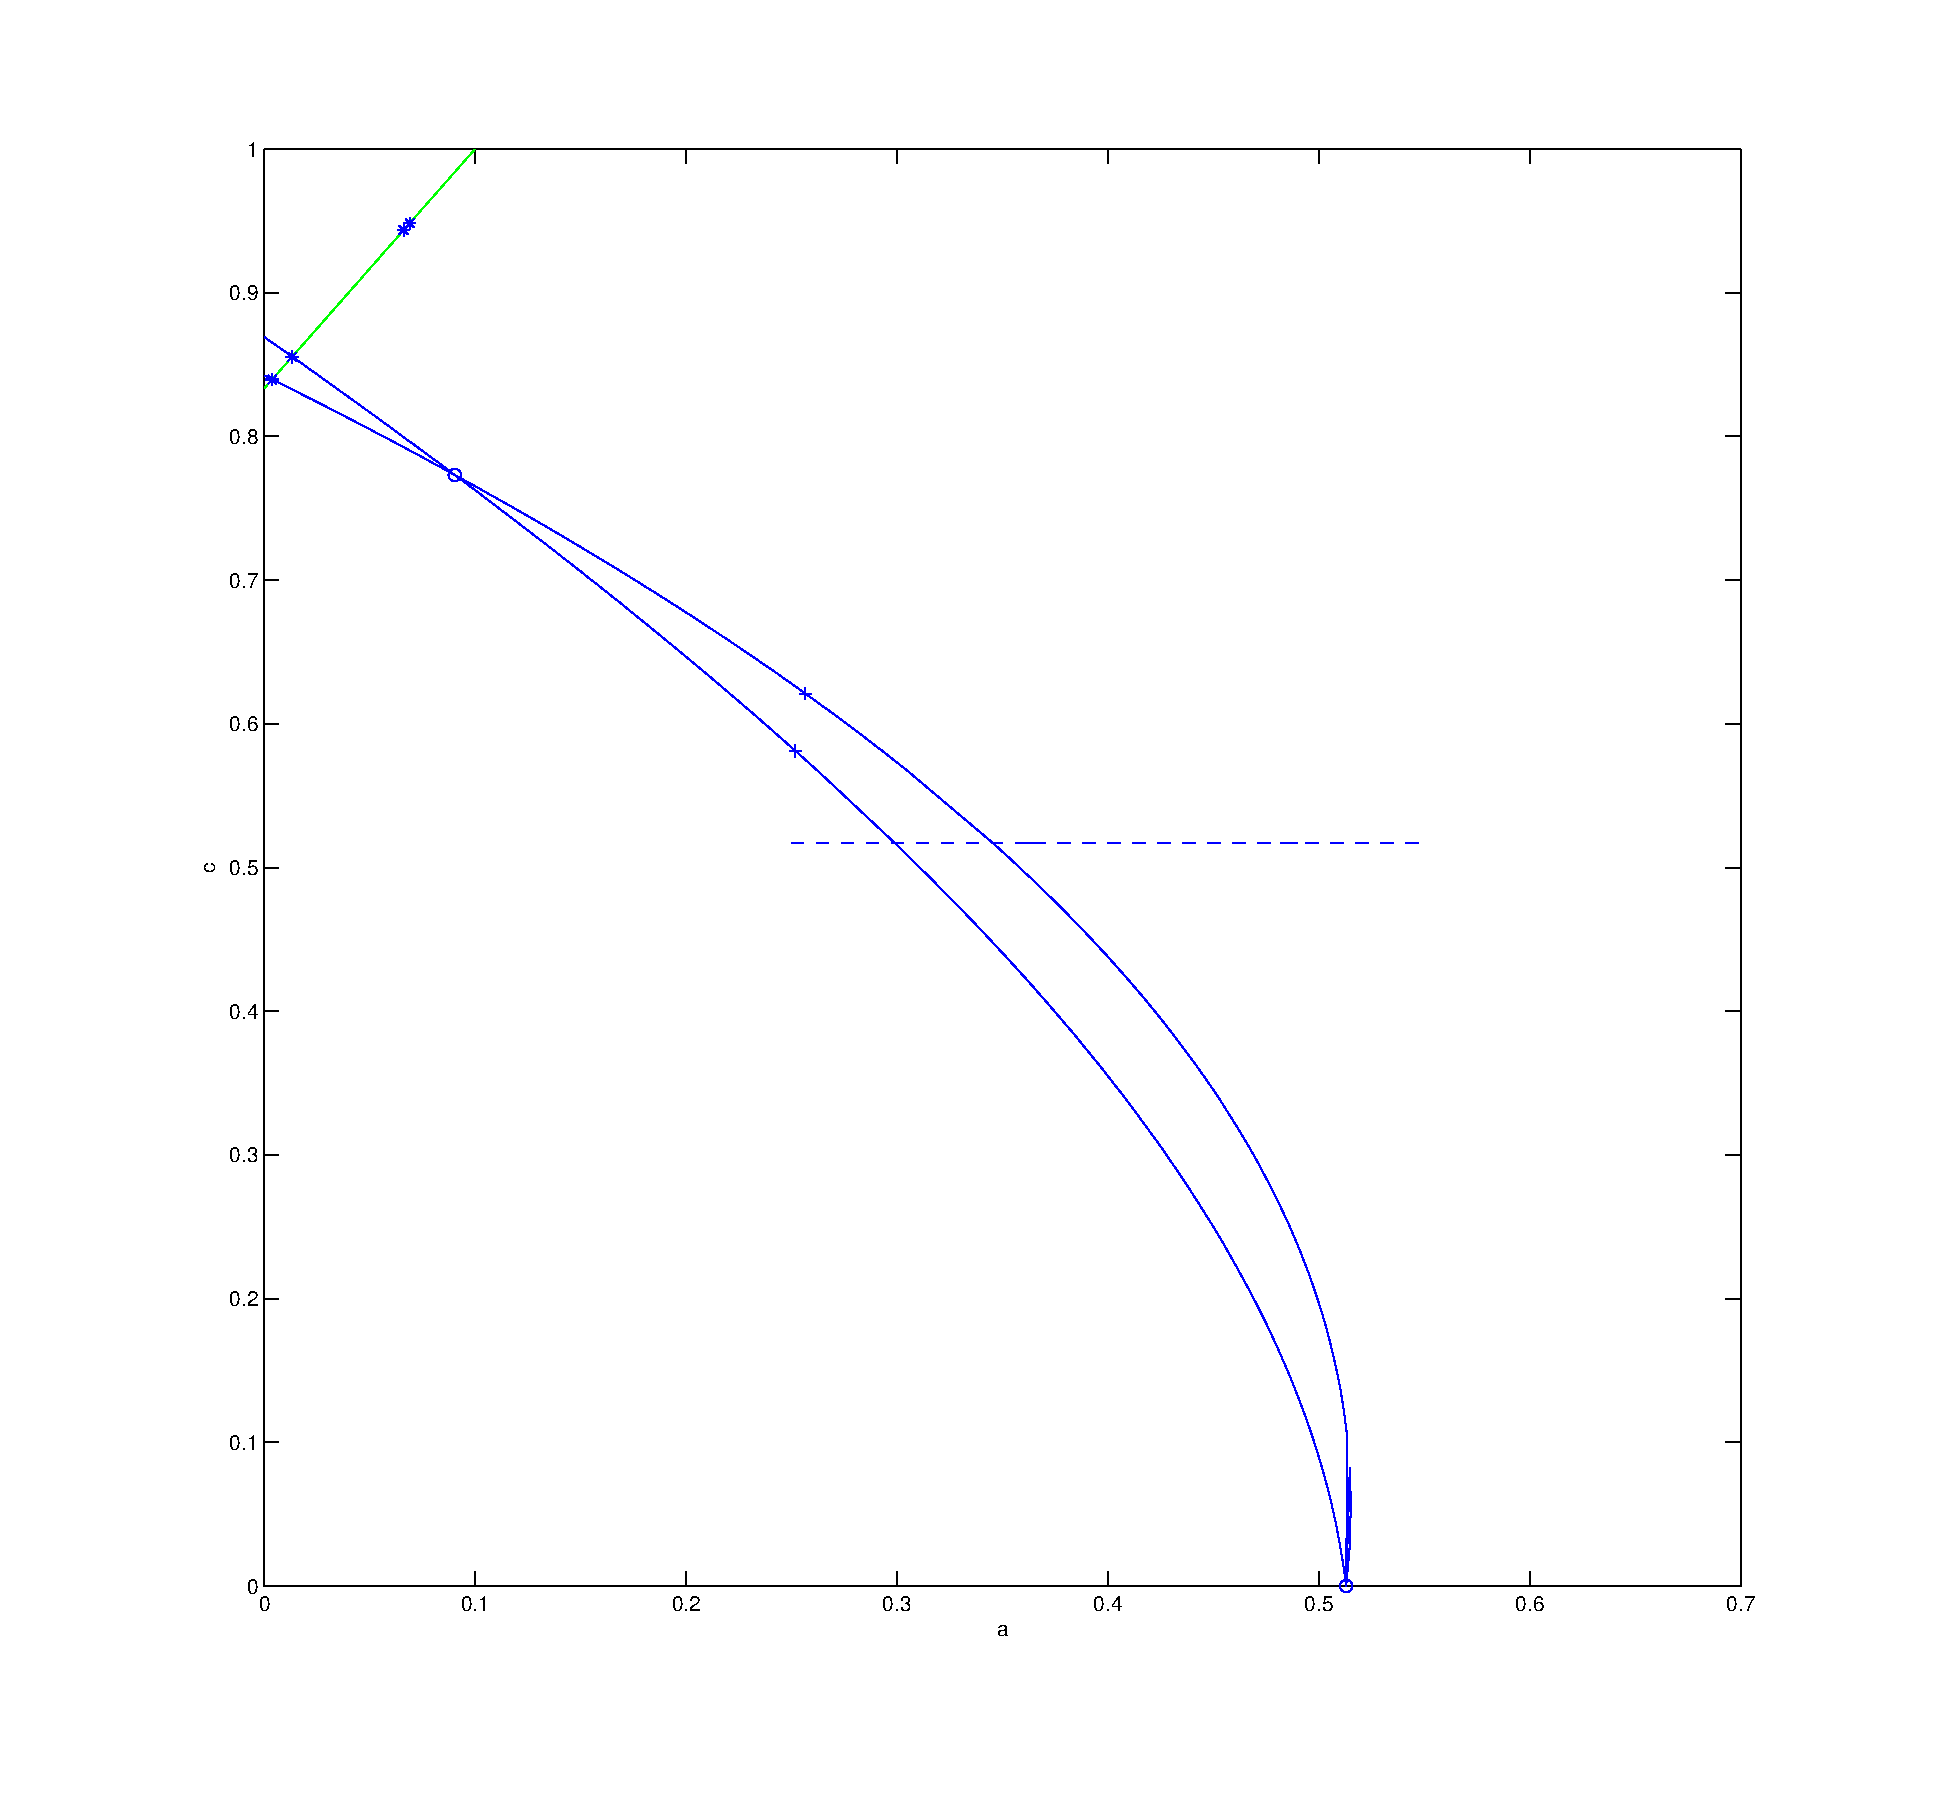
\includegraphics[scale=0.4]{images/nmfm_demo_02}\caption{Plot of detected bifurcations on the fold and Hopf branches. The asterisks
'\textcolor{blue}{{*}}' indicates fold-Hopf bifurcations, the open
circle '\textcolor{blue}{o}' indicates a double-Hopf, the plus '\textcolor{blue}{+}'
indicates generalized Hopf. \label{fig:Plot-of-Hopf-branches}}
\end{figure}





\section{Example with Bogdanov-Takens bifurcation\label{sec:Example2}}

In \cite{liu2013bogdanov} the Bogdanov-Takens bifurcation of the
following delayed predator prey system

\begin{equation}
\left\{ \begin{array}{rl}
\dot{x} & =rx\left(1-\dfrac{x}{K}\right)-\dfrac{\alpha y(x-\bar{m})}{Ay+x-\bar{m}}-\bar{h,}\\
\dot{y} & =sy\left(1-\dfrac{dy(t-\bar{\tau})}{x(t-\bar{\tau})-\bar{m}}\right),
\end{array}\right.\label{eq:Holling-Tanner-1}
\end{equation}
is considered. Here $x$ and $y$ stand for prey and predator population
(or densities) at time $t$, respectively. The predator growth is
of logistic type with growth rate r and carrying capacity $K$ in
the absence of predation; $\lyxmathsym{\textgreek{a}}$ and $A$ stand
for the predator capturing rate and half saturation constant, respectively;
$s$ is the intrinsic growth rate of predator; however, carrying capacity
$x/b$ ($b$ is the conversion rate of prey into predators) is the
function on the population size of prey. The parameters $\lyxmathsym{\textgreek{a}},A,\bar{m},\bar{h},s,b,$
and $\bar{\lyxmathsym{\textgreek{t}}}$ are all positive constants.
$\bar{m}$ is a constant number of prey using refuges; $h$ is the
rate of prey harvesting. System (\ref{eq:Holling-Tanner-1}) can be
transformed into
\begin{equation}
\left\{ \begin{array}{rl}
\dot{x} & =(x+m)(1-x-m)-\dfrac{xy}{ay+x}-h,\\
\dot{y} & =\delta y\left(\beta-\dfrac{y(t-\tau)}{x(t-\tau)}\right),
\end{array}\right.\label{eq:Holling-Tanner-1-1}
\end{equation}
see \cite{liu2013bogdanov} for the transformation and the meaning
of the new parameters. 

Let 
\begin{equation}
\begin{aligned}0<m<\dfrac{1}{2}\left(1-\dfrac{\beta}{a\beta+1}\right),\\
h=\dfrac{1}{4}\left(\dfrac{\beta}{a\beta+1}-1\right)^{2}+\dfrac{m\beta}{a\beta+1}.
\end{aligned}
\label{eq:conditions_mh}
\end{equation}


\noindent Then $P_{*}=(x_{*},y_{*})$ is an interior positive equilibrium
point of systems (\ref{eq:Holling-Tanner-1-1}), where
\begin{equation}
x_{*}=-\frac{1}{2}\left(\frac{\beta}{a\beta+1}+2m-1\right),\qquad y_{*}=\beta x_{*}.\label{eq:steady-state}
\end{equation}
In order to discuss the properties of system (\ref{eq:Holling-Tanner-1-1})
in the neighborhood of the equilibrium point $P_{\ast}=(x_{\ast},y_{\ast})$,
let $x=x\lyxmathsym{\textminus}x_{\ast}$, $y=y\lyxmathsym{\textminus}y_{\ast}$;
then $P_{\ast}$ is translated to $(0,0)$, and the linearization
of system (\ref{eq:Holling-Tanner-1-1}) becomes (still denoting $\bar{x},\ \bar{y}$
as $x,\ y$)
\begin{equation}
\left\{ \begin{aligned}\dot{x} & =\dfrac{\tau\beta}{\left(a\beta+1\right)^{2}}x-\dfrac{\tau}{\left(a\beta+1\right)^{2}}y,\\
\dot{y} & =\tau\delta\beta^{2}x(t-1)-\tau\delta\beta y(t-1).
\end{aligned}
\right.\label{eq:linearized}
\end{equation}
Here we have rescaled the time as $t\rightarrow\dfrac{t}{\tau}$,
so that $\tau$ can be treated as an ordinary parameter. Denoting
$\mathbf{x}\equiv(x,y)$ system (\ref{eq:linearized}) can be written
as
\[
\dot{\mathbf{x}}=\dfrac{\tau}{\left(a\beta+1\right)^{2}}\left(\begin{array}{cc}
\beta & -1\\
0 & 0
\end{array}\right)\mathbf{x}+\tau\delta\beta\begin{pmatrix}0 & 0\\
\beta & -1
\end{pmatrix}\mathbf{x}(t-1).
\]
The characteristic matrix becomes
\[
\Delta(\lambda)=\begin{pmatrix}\lambda-\dfrac{\tau\beta}{\left(a\beta+1\right)^{2}} & \dfrac{\tau}{\left(a\beta+1\right)^{2}}\\
-\tau\delta\beta^{2}e^{-\lambda} & \lambda+\tau\delta\beta e^{-\lambda}
\end{pmatrix}.
\]
It follows that the characteristic equation of (\ref{eq:linearized})
is given by
\begin{equation}
\det(\Delta(\lambda))=\lambda^{2}+\beta\tau\left(\delta e^{-\lambda\tau}-\dfrac{1}{\left(a\beta+1\right)^{2}}\right)\lambda.\label{eq:chareq}
\end{equation}
Expanding (\ref{eq:chareq}) around $\lambda=0$ yields
\[
\det(\Delta(\lambda))=\beta\tau\left(\delta-\frac{1}{(a\beta+1)^{2}}\right)\lambda+2\left(1-\beta\delta\tau\right)\lambda^{2}+\mathcal{O}(\lambda^{3}).
\]


\noindent Clearly, if
\begin{equation}
\begin{array}{c}
\delta=\dfrac{1}{\left(a\beta+1\right)^{2}},\\
\tau\neq\dfrac{1}{\delta\beta},\qquad\text{that is,}\qquad\tau\neq\dfrac{\left(a\beta+1\right)^{2}}{\beta};
\end{array}\label{eq:example2_delta_bt_point}
\end{equation}
then $\lambda=0$ is a double zero eigenvalue.

We now assume that we are at a Bogdanov-Takens point such that (\ref{eq:example2_delta_bt_point})
are satisfied. Then the vectors
\begin{align*}
q_{0} & =\left(\frac{1}{\sqrt{\beta^{2}+1}},\frac{\beta}{\sqrt{\beta^{2}+1}}\right)^{T},\\
q_{1} & =\left(\frac{a^{2}\beta-\frac{\beta\tau^{2}}{2(a\beta+1)^{2}-2\beta\tau}+2a+\frac{1}{\beta}-\tau}{\sqrt{\beta^{2}+1}},\frac{\beta\tau\left(\beta\tau-2(a\beta+1)^{2}\right)}{2\sqrt{\beta^{2}+1}\left((a\beta+1)^{2}-\beta\tau\right)}\right)^{T},\\
p1 & =\left(\frac{\beta\sqrt{\beta^{2}+1}}{(a\beta+1)^{2}-\beta\tau},-\frac{\sqrt{\beta^{2}+1}}{(a\beta+1)^{2}-\beta\tau}\right)^{T},\\
p_{0} & =\left(0,\frac{\sqrt{\beta^{2}+1}}{\beta}\right)^{T},
\end{align*}
satisfy the relations (\ref{eq:bt_jordanchains}) and (\ref{eq:bt_normalized_eigenvectors}).
Using a computer algebra system like \texttt{Mathematica}, the coefficients
in (\ref{eq:bt_coef}) become 
\begin{equation}
\begin{aligned}a & =-\dfrac{\beta}{\sqrt{\beta^{2}+1}\left((a\beta+1)^{2}-\beta\tau\right)},\\
b & =\dfrac{4\beta\tau(a\beta+1)^{2}-2(a\beta+1)^{4}-\beta^{2}\tau^{2}}{\sqrt{\beta^{2}+1}\left((a\beta+1)^{2}-\beta\tau\right)^{2}}.
\end{aligned}
\label{eq:example2_coef_ab}
\end{equation}
We note that although these coefficients are slightly different from
the coefficients derived in \cite{liu2013bogdanov}, the sign of the
product of $ab$ remains the same. Here we choose to normalize the
vector $q_{0}$ to have length 1, as done in the Matlab scripts, see
the file \blist{p\_tobt.m}. Furthermore, the coefficients here have
been derived from system (\ref{eq:Holling-Tanner-1-1}) directly,
whereas in \cite{liu2013bogdanov} first the time as been rescaled
by $t\rightarrow\dfrac{t}{\tau}$.

The files of this demonstration are located in the folder \texttt{demos/Holling-Tanner
}of the DDE-BifTool package.


\subsection{Generating system files for DDE-BifTool}

\noindent To generate the system files\textbf{ }we again use the \texttt{Maple}
script \texttt{Maple\_gen\_sys.mw}\textbf{.} We only display the file
\blist{sys\_rhs.m}\textbf{ }here, since the files \blist{sys\_deri}
and \blist{sys\_mfderi} are too long
\begin{lstlisting}[basicstyle={\footnotesize},breaklines=true,language=Matlab,tabsize=4]
function f = sys_rhs(xx,par)

f(1,1) = (xx(1,1)+par(4))*(1-xx(1,1)-par(4))-...
	xx(1,1)*xx(2,1)/(par(3)*xx(2,1)+xx(1,1))-par(5);
f(2,1) = par(6)*xx(2,1)*(par(1)-xx(2,2)/xx(1,2));

end 
\end{lstlisting}



\subsection{Initialization of the system in DDE-BifTool}

We add the necessary paths to our workspace so that we can access
the script files of \texttt{ddebiftool}, \texttt{ddebiftool\_utilities},
\texttt{ddebiftool\_extra\_nmfm}. We also add the extension \\
\texttt{ddebiftool\_extra\_psol} for the continuation of the homoclinic
orbit emanating from the Bogdanov-Takens point .

\begin{lstlisting}[basicstyle={\footnotesize},breaklines=true,language=Matlab,tabsize=4]
clear;
close all;
addpath('../../../ddebiftool',...
	'../../../ddebiftool_extra_psol',...
	'../../../ddebiftool_extra_nmfm',...
	'../../../ddebiftool_utilities');
funcs=set_funcs(...
	'sys_rhs', @(xx,par) sys_rhs(xx,par),...
	'sys_tau', @() 2,... 
	'sys_deri', @(xx,par,nx,np,v) sys_deri(xx,par,nx,np,v),...
	'sys_mfderi',@(xx,par,varargin) sys_mfderi(xx,par,varargin{:}));

disp('Holling-Tanner');
% par=(beta,tau,a,m,h,delta)
\end{lstlisting}



\subsection{Continuation of steady-state branch}

We fixed the parameters 

\begin{equation}
\begin{array}{l}
a=0.5,\qquad\tau=0.78125,\qquad m=0.02,\\
h=0.098,\qquad\beta=0.4,\qquad\delta=0.54089.
\end{array}\label{eq:example2_fixedparameters}
\end{equation}
Then we continue the positive steady-state (\ref{eq:steady-state})
in $\beta$.

\begin{lstlisting}[basicstyle={\footnotesize},breaklines=true,language=Matlab,tabsize=4]
beta=0.5;a=0.5; 
m=(1/30)*(1-beta/(a*beta+1)); 
h=(1/4)*(beta/(a*beta+1)-1)^2+m*beta/(a*beta+1); 
tau=1/4*(a*beta+1)^2/beta; delta=1/(a*beta+1)^2;

beta=0.4;
delta=0.5409; 

stst.parameter=[beta,tau,a,m,h,delta];

xster=-(1/2)*((beta/(a*beta+1)+2*m-1)+...
		sqrt((1-2*m-beta/(a*beta+1))^2+4*(m*(1-m)-h)));
yster=beta*xster;

contpar=1; 
stst_branch = SetupStst(funcs,'x',[xster; yster],'parameter',stst.parameter,...
    'contpar',contpar,'max_step',[contpar 0.02],'min_bound',...     
	[contpar 0.4],'max_bound',[contpar 0.6],...     
	'newheuristics_tests',0);

stst_branch.method.continuation.plot = 1;

[stst_branch,s,f,r] = br_contn(funcs,stst_branch,100); 

stst_branch.method.bifurcation.monitor_eigenvalues=0; 
stst_branch.method.bifurcation.plot_testfunctions=1; 
stst_branch.method.bifurcation.pause_on_bifurcation=0;

stst_branch = br_stabl(funcs,stst_branch,0,0);
stst_branch=br_bifdet(funcs,stst_branch);
\end{lstlisting}
Running the above code outputs:

\begin{Verbatim}[commandchars=\\\{\},fontsize=\scriptsize]
BR_CONTN warning: boundary hit. 

BR_BIFDET: Fold detected near par(1) = 0.4998182859. 
BR_BIFDET: Fold located at  par(1) = 0.5000000000. 
BR_BIFDET: Normal form coefficient: b = 4.8721895296

BR_BIFDET: Hopf detected near par(1) = 0.4916389145. 
BR_BIFDET: Hopf located at  par(1) = 0.4939507149. 
BR_BIFDET: Normal form coefficient: L1 = 192.7259505902
\end{Verbatim}

In Figure \ref{fig:stst_branch} we have plotted the continuation
of the steady-state branch and the test functions $\psi_{f}$ and
$\psi_{H}$.

\begin{figure}[h]
\centering{}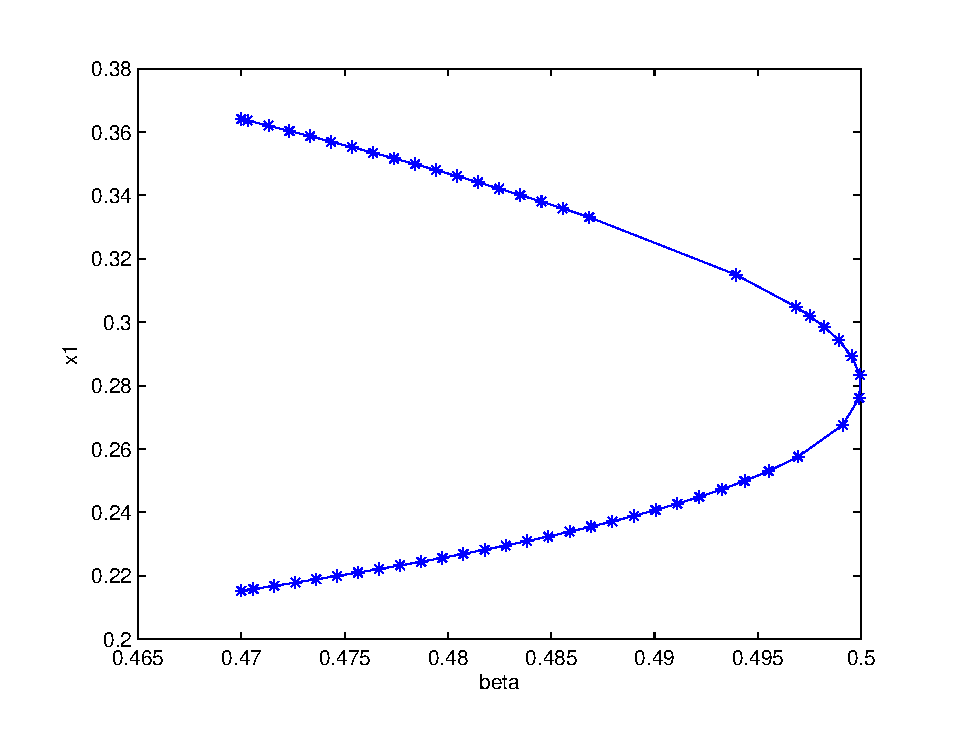
\includegraphics[scale=0.4]{images/continuation_stst_branch_plot}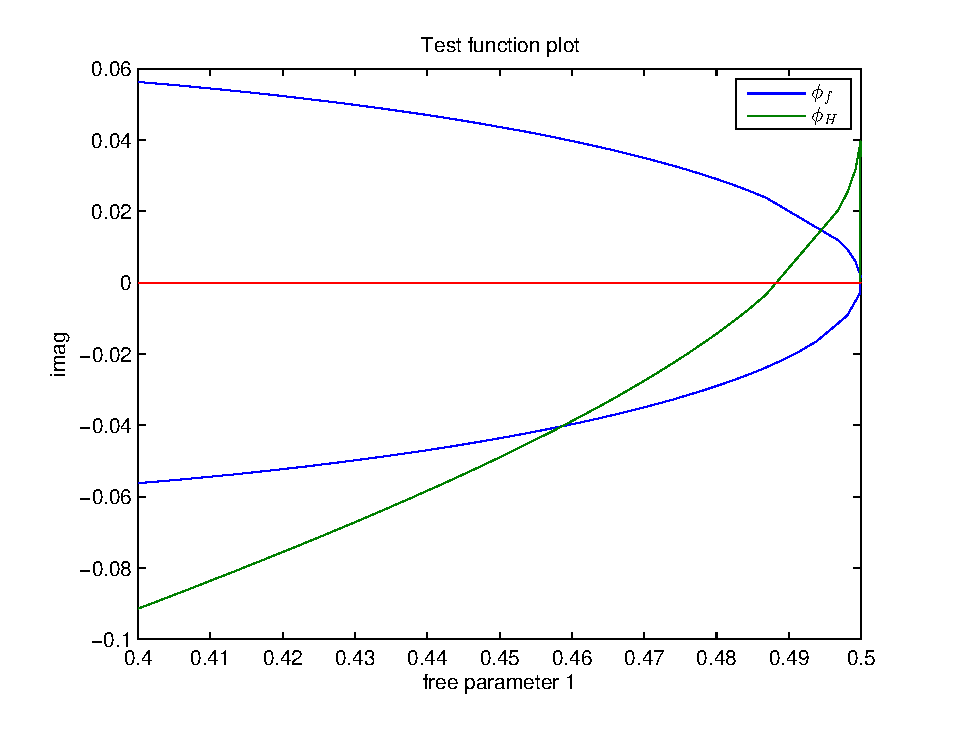
\includegraphics[scale=0.4]{images/exm2_stst_br_testfunctions}\caption{Left is a plot of the continuation of the steady-state point. In the
right figure the test functions are plotted. Here we see that the
Hopf bifurcation is near the fold bifurcation, as predicted by a Bogdanov-Takens
bifurcation. \label{fig:stst_branch}}
\end{figure}



\subsection{Continuation of the Hopf point}

We continue the detected Hopf point at $\beta=0.4886954168$ in $(\beta,\delta)$

\begin{lstlisting}[basicstyle={\footnotesize},breaklines=true,language=Matlab,tabsize=4]
FPI = br_getflags(stst_branch); 
start_ind = FPI(1);

% We do a standard continuation, using the starting index obtained from the 
% flagged point indices.
fprintf('----- Hopf branch -----\n'); 
[hopf_branch, suc] = SetupHopf(funcs, stst_branch, start_ind,...     
	'contpar', [1 6], 'dir', 1, 'step', 0.002);

betamin=0.4; betamax=0.6; deltamin=0.4; deltamax=0.7;

hopf_branch.parameter.min_bound=[1 betamin; 6 deltamin]; 
hopf_branch.parameter.max_bound=[1 betamax; 6 deltamax]; 
hopf_branch.parameter.max_step=[1 0.0005; 6 0.0005];

hopf_branch.method.stability.minimal_time_step = 0.005; % default 0.01
[hopf_branch,s,f,r]=br_contn(funcs,hopf_branch,250);
\end{lstlisting}
In Figure \ref{fig:hopf_branch} we see two plots of the Hopf branch.
In the first plot we have plotted the two continuation parameters
$\beta$ against $\delta$. In the second plot we have plotted the
point number along the branch versus $\delta$. From the two graphs
we conclude that the Hopf curve makes a turn at $(\beta,\delta)\approx(0.5,0.64)$.

\begin{figure}[H]
\begin{centering}
\includegraphics[scale=0.4]{images/hopf_branch}\includegraphics[scale=0.4]{images/hopf_branch_pointnumber_vs_delta}
\par\end{centering}

\centering{}\caption{Left is a plot of the continuation of the steady-state point. At the
right side we see a plot of the point number along the branch versus
$\delta$. \label{fig:hopf_branch}}
\end{figure}


In Figure \ref{fig:example2_test_functions_hopf_branch} we have plotted
the test functions. We see that the test function for a Bogdanov-Takens
point on a Hopf curve passes 0 even when the parameters make a turn.

\begin{figure}[h]
\noindent \begin{centering}
\includegraphics[scale=0.6]{images/exm2_hopfbr1_testfunctions}
\par\end{centering}

\caption{Plot of the test function along\protect\blist{hopf\_branch}. \label{fig:example2_test_functions_hopf_branch}}


\end{figure}



\subsection{Detection on the Hopf branch}

We use the function \blist{br\_bifdet} to detect bifurcations on
the Hopf branch

\begin{Verbatim}[commandchars=\\\{\},fontsize=\scriptsize]
>> hopf_branch = br_stabl(funcs,hopf_branch,0,0); 
>> [hopf_branch,success] = br_bifdet(funcs,hopf_branch);
BR_BIFDET: Bogdanov-Takens detected near par(1) = 0.4999998471, par(6) = 0.6395308481. 
BR_BIFDET: a = -0.3812625439, b = -1.6892715659, par(1) = 0.5000000000, par(6) = 0.6400000000.
\end{Verbatim}

As predicted we see a Bogdanov-Takens point (BT point) located at
$(\beta,\delta)=(0.5,0.64)$. From the normal form coefficients we
conclude that the Hopf bifurcation generates an unstable limit cycle.
Combining $(\beta,\delta)=(0.5,0.64)$ with (\ref{eq:example2_fixedparameters})
we confirm that the equations for a Bogdanov-Takens point derived
analytically in (\ref{eq:example2_delta_bt_point}) and the coefficients
in (\ref{eq:example2_coef_ab}) are satisfied.


\subsection{Direct calculation of the Bogdanov-Takens normal form coefficients}

Since in this example we know the position of the Bogdanov-Takens
through analytic calculations, we could calculate the normal form
coefficients directly as shown below. 

\begin{lstlisting}[basicstyle={\footnotesize},breaklines=true,language=Matlab,tabsize=4]
beta=0.5;a=0.5; 
m=(1/30)*(1-beta/(a*beta+1)); 
h=(1/4)*(beta/(a*beta+1)-1)^2+m*beta/(a*beta+1); 
tau=1/4*(a*beta+1)^2/beta; 
delta=1/(a*beta+1)^2;

xster=-(1/2)*(beta/(a*beta+1)+2*m-1); 
yster=beta*xster;

p.kind='stst'; 
p.parameter=[beta,tau,a,m,h,delta]; 
p.x=[xster;yster];

bt=p_tobt(funcs,p); 
bt=nmfm_bt(funcs,bt); 
bt.nmfm
\end{lstlisting}
The last line gives the following output:

\begin{Verbatim}[commandchars=\\\{\},fontsize=\scriptsize]
ans = 
	a2: -0.3816     
	b2: -1.6895
\end{Verbatim}

Here $a=a_{2}$ and $b=b_{2}$.


\subsection{Continue fold point}

We will continue the fold point detected on the steady-state.
\begin{lstlisting}[basicstyle={\footnotesize},breaklines=true,language=Matlab,tabsize=4]
FPI = br_getflags(stst_branch); 
start_ind = FPI(bif2num('fold'),1);

[fold_branch, suc] = SetupFold(funcs, stst_branch, start_ind, ...
    'contpar', [1 6], 'dir', 6, 'step', 0.005);
betamin=0.4; betamax=0.6; deltamin=0.3; deltamax=0.7;

fold_branch.parameter.min_bound=[1 betamin; 6 deltamin]; 
fold_branch.parameter.max_bound=[1 betamax; 6 deltamax]; 
fold_branch.parameter.max_step=[1 0.005; 6 0.005];

[fold_branch,s,f,r]=br_contn(funcs,fold_branch,300); 
fold_branch = br_rvers(fold_branch); 
[fold_branch,s,f,r]=br_contn(funcs,fold_branch,300);

fold_branch = br_stabl(funcs,fold_branch,0,0); 
[fold_branch,success] = br_bifdet(funcs,fold_branch);
\end{lstlisting}


In the Matlab console the following output is given:

\begin{Verbatim}[commandchars=\\\{\},fontsize=\scriptsize]
BR_CONTN warning: boundary hit. 
BR_CONTN warning: boundary hit. 

BR_BIFDET: Cusp detected near par(1) = 0.5000000000, par(6) = 0.6387723214. BR_BIFDET: 
Failed to correct cusp.

BR_BIFDET: Bogdanov-Takens detected near par(1) = 0.5000000000, par(6) = 0.6387723214. 
BR_BIFDET: a = -0.3812625439, b = -1.6892715659, par(1) = 0.5000000000, par(6) = 0.6400000000.
\end{Verbatim}

Why there is a falsely detected cusp at near the Bogdanov-Takens point
is explained in the next Section, where we treat the cusp bifurcation
in detail.


\subsection{Homoclinic orbit}

We continue the periodic orbit emanating from the Hopf curve in $\delta$

\begin{lstlisting}[basicstyle={\footnotesize},breaklines=true,language=Matlab,tabsize=4]
hopf=hopf_branch.point(20); 
[psol,stp]=p_topsol(funcs,hopf,1e-2,3,27);

ind_delta=6; 
mpsol=df_mthod(funcs,'psol'); 
[psol,s]=p_correc(funcs,psol,ind_delta,stp,mpsol.point); 
psol_branch=df_brnch(funcs,ind_delta,'psol'); 
psol_branch.point=psol; 
[psol,stp]=p_topsol(funcs,hopf,1.1e-2,3,27); 
[psol,s]=p_correc(funcs,psol,ind_delta,stp,mpsol.point); 
psol_branch.point(2)=psol; 

figure(2);clf; 
[xm,ym]=df_measr(0,psol_branch); 
ym.field='period'; 
ym.col=1; 
ym.row=1; 
psol_branch.method.continuation.plot_measure.x=xm; 
psol_branch.method.continuation.plot_measure.y=ym; 
[psol_branch,s,r,f]=br_contn(funcs,psol_branch,40); 

xlabel('$\delta$','interpreter','latex');
ylabel('period');
\end{lstlisting}
In Figure \ref{fig:limit-cycle} we have plotted $\delta$ against
the period of the limit cycle. Around $\delta\approx0.577$ the period
goes to infinity, indicating a homoclinic orbit.

\begin{figure}
\begin{centering}
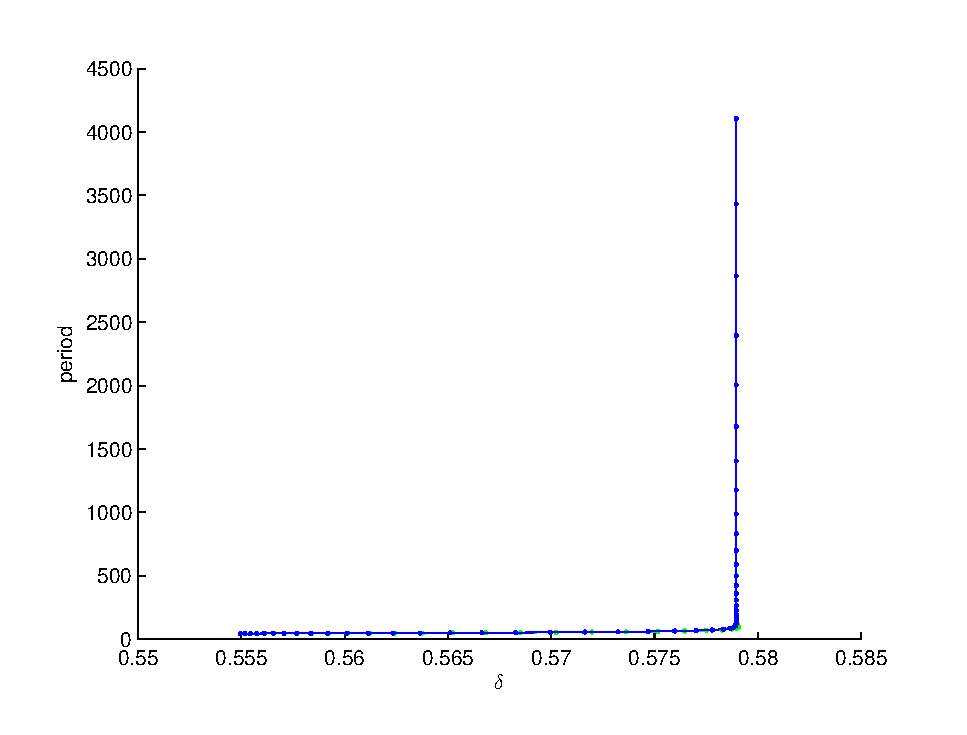
\includegraphics[scale=0.6]{images/limitcycle_period}
\par\end{centering}

\caption{Plot of the cycle emanating from the Hopf curve. At $\delta\approx0.577$
the period of the cycles goes to infinity, indicating a homoclinic
obit.\label{fig:limit-cycle}}
\end{figure}
We select the last cycle on the \blist{psol\_branch} and convert
it to a homoclinic orbit. Then we continue the homoclinic orbit in
$(\beta,\delta)$
\begin{lstlisting}[basicstyle={\footnotesize},breaklines=true,language=Matlab,tabsize=4]
psol=psol_branch.point(end);
hcli=p_tohcli(funcs,psol);

mhcli=df_mthod(funcs,'hcli');
[hcli,s]=p_correc(funcs,hcli,ind_delta,[],mhcli.point);	% correct
hcli=p_remesh(hcli,3,50);	% remesh it and 
[hcli,s]=p_correc(funcs,hcli,ind_delta,[],mhcli.point)	% correct it again

%% perturb hcli, correct and continue ind_beta=1; 
hcli_br=df_brnch(funcs,[ind_beta, ind_delta],'hcli'); 
hcli_br.point=hcli; 
hcli.parameter(ind_beta)=hcli.parameter(ind_beta)-6e-6; 
[hcli,s]=p_correc(funcs,hcli,ind_delta,[],mhcli.point); 
hcli_br.point(2)=hcli;

figure(1); 
[hcli_br,s,r,f]=br_contn(funcs,hcli_br,28); 
hcli_br=br_rvers(hcli_br); 
[hcli_br,s,r,f]=br_contn(funcs,hcli_br,40);

xlabel('$\beta$','interpreter','latex'); 
ylabel('$\delta$','interpreter','latex');
\end{lstlisting}
In Figure \ref{fig:homoclinic-orbit} we see the homoclinic orbit
continued.

\begin{figure}
\begin{centering}
\includegraphics[scale=0.6]{images/homoclinic_branch}
\par\end{centering}

\caption{Continuation of the homoclinic orbit in $(\beta,\delta)$.\label{fig:homoclinic-orbit}}
\end{figure}



\subsection{Stability of the cycles}

The following code calculates the stability of the cycles from \blist{psol\_branch}.

\begin{lstlisting}[basicstyle={\footnotesize},breaklines=true,language=Matlab,tabsize=4]
psol_branch = br_stabl(funcs,psol_branch,0,0);
\end{lstlisting}


In the field \blist{psol\_branch.point(i).stability.mu} the multipliers
for the $i$th point on the branch are given. In Figure \ref{fig:exam2_multipliers}
we have plotted the multipliers for point number 10. There we see
that the cycle is indeed unstable as predicted by the product of the
coefficients $ab>0$.

\begin{figure}
\noindent \begin{centering}
\includegraphics[width=0.8\textwidth]{images/exm2_psol_br_multipliers}
\par\end{centering}

\caption{Multipliers for point number 10 from \protect\blist{psol\_branch}.\label{fig:exam2_multipliers}}


\end{figure}



\subsection{Bifurcation diagram}

In Figure \ref{fig:bifurcation_diagram} we have plotted the fold
branch as well as the homoclinic and the Hopf branch, giving a complete
bifurcation diagram of the Bogdanov-Takens point.

\begin{figure}[H]
\begin{centering}
\includegraphics[width=0.8\textwidth]{images/bifurcation_diagram}
\par\end{centering}

\caption{Plot of Hopf, homoclinic and fold branch emanating from the Bogdanov-Takens
point. \label{fig:bifurcation_diagram}}
\end{figure}



\section{Example with cusp and Bogdanov-Takens bifurcations\label{sec:Example3}}

In this last example we will consider the mathematical model 
\begin{equation}
\begin{cases}
\mu\dot{u}_{1}(t)=-u_{1}(t)+q_{11}\alpha(u_{1}(t\text{-}T))-q_{12}u_{2}(t\text{-}T)+e_{1},\\
\mu\dot{u}_{2}(t)=-u_{2}(t)+q_{21}\alpha(u_{1}(t\text{-}T))-q_{22}u_{2}(t\text{-}T)+e_{2},
\end{cases}\label{eq:neural_network}
\end{equation}
which describes the dynamics of a neural network consisting of an
excitatory and inhibitory neuron \cite{giannakopoulos2001bifurcations}.
The variables and parameters occurring in (\ref{eq:neural_network})
have the following neurophysiological meaning:
\begin{itemize}
\item $u_{1},u_{2}:\mathbb{R}\rightarrow R$ denote the total post-synaptic
potential of the excitatory and inhibitory neuron, respectively.
\item $\mu>0$ is a time constant characterizing the dynamical properties
of cell membrane.
\item $q_{ik}\geq0$ represents the strength of the connection line from
the $k$th neuron to the $i$th neuron.
\item $\alpha:\mathbb{R}\rightarrow\mathbb{R}$ is the transfer function
which describes the activity generation of the excitatory neuron as
a function of its total potential $u_{1}$. The function $\alpha$
is smooth, increasing and has an unique turning point at $u_{1}=\theta$.
The transfer function corresponding to the inhibitory neuron is assumed
to be the identity.
\item $T\geq0$ is a time delay reflecting synaptic delay, axonal and dendritic
propagation time.
\item $e_{1}$ and $e_{2}$ are external stimuli acting on the excitatory
and inhibitory neuron, respectively.
\end{itemize}
We consider equation (\ref{eq:neural_network}) with
\begin{align*}
\alpha(u_{1}) & =\frac{1}{1+e^{-4u_{1}}}-\frac{1}{2},\qquad q_{11}=2.6,\qquad q_{21}=1.0,\qquad q_{22}=0.0,\\
\mu & =1.0,\qquad T=1.0,\qquad e_{2}=0.0,
\end{align*}
and $Q:=q_{12},\, E:=e_{1}$ as bifurcation parameters. Substituting
into (\ref{eq:neural_network}) yields
\begin{equation}
\begin{cases}
\dot{u}_{1}(t)=-u_{1}(t)+2.6\alpha(u_{1}(t\text{-}T))-Qu_{2}(t\text{-}T)+E,\\
\dot{u}_{2}(t)=-u_{2}(t)+\alpha(u_{1}(t\text{-}T)).
\end{cases}\label{eq:neural_network_subs}
\end{equation}
A steady-state solution of (\ref{eq:neural_network_subs}) is given
by $(u_{1},u_{2})\equiv(0,0)$ with $E=0$ and $Q$ arbitrary. 

The files of this demonstration are located in the folder \texttt{demos/cusp
}of the DDE-BifTool package.


\subsection{Initialization}

As before we start by loading the necessary script files and setting
the \blist{funcs} structure.

\begin{lstlisting}[basicstyle={\footnotesize},language=Matlab,tabsize=4]
%% setup system clear all;
clear variables close all;
close figures addpath('../../ddebiftool',...
    '../../ddebiftool_extra_psol',...
    '../../ddebiftool_extra_nmfm',...
    '../../ddebiftool_utilities');

funcs=set_funcs(...
    'sys_rhs', @(xx,par) sys_rhs(xx,par),...
    'sys_tau', @() 6,...
    'sys_deri', @(xx,par,nx,np,v) sys_deri(xx,par,nx,np,v),...
    'sys_mfderi',@(xx,par,varargin) sys_mfderi(xx,par,varargin{:}));
\end{lstlisting}



\subsection{Continuation of steady state point}

We continue the steady state $(u_{1},u_{2})\equiv(0,0)$ at $(Q,E)=(0,0)$
in $Q$:

\begin{lstlisting}[basicstyle={\footnotesize},language=Matlab]
Q=0; E=0;
q11=2.6; q12=Q; q21=1; e1=E; e2=0; T=1;
par = [q11,q12,q21,e1,e2,T];

stst_br = SetupStst(funcs,'x',[0;0],'parameter',par,...
	'contpar',4,'max_step',[4 0.02],'max_bound',[4 1],'min_bound',[4 0],...
    'newheuristics_tests',0);

[stst_br,s,f,r] = br_contn(funcs,stst_br,300);

stst_br=br_stabl(funcs,stst_br,0,0);
stst_br=br_bifdet(funcs,stst_br); 
\end{lstlisting}
In the matlab console the following output is given:

\begin{Verbatim}[commandchars=\\\{\},fontsize=\scriptsize]
BR_CONTN warning: boundary hit. 
BR_BIFDET: Fold detected near par(4) = 0.4899601374. 
BR_BIFDET: Fold located at  par(4) = 0.4913668450. 
BR_BIFDET: Normal form coefficient: b = 0.7321765321
\end{Verbatim}

\noindent In Figure \ref{fig:stst_br_testfunctions} we have plotted
the test functions $\psi_{f}$ and $\psi_{H}$.

\begin{figure}[h]
\centering{}\includegraphics[width=1\textwidth]{images/exm3_stst_testfunctions}\caption{Plot of test function for stst\_br\label{fig:stst_br_testfunctions}}
\end{figure}
The discontinuity in the test function for a Hopf point $\phi_{H}$
is produced, since the only complex eigenvalues pass the default lower
bound of -1 when calculating the eigenvalues of the points on the
steady-state points. This can be seen by monitoring the eigenvalues
on the steady-state branch by calling 
\begin{lstlisting}[basicstyle={\footnotesize},language=Matlab]
stst_br.method.bifurcation.plot_testfunctions = 1;
stst_br.method.bifurcation.monitor_eigenvalues = 0;
stst_br=br_bifdet(funcs, stst_br);
\end{lstlisting}
By setting \blist{stst\_br.method.stability.minimal\_real\_part=-5}
before calculating the stability along the steady-state branch we
get a smooth curve for $\psi_{H}$, see Figure (\ref{fig:stst_br_testfunctions_smooth}).

\begin{figure}[h]
\centering{}\includegraphics[width=1\textwidth]{images/exm3_stst_testfunctions_smooth}\caption{Plot of test functions for stst\_br\label{fig:stst_br_testfunctions_smooth}}
\end{figure}



\subsection{Continuation of the Fold point and detecting codim-2 bifurcations}

We continue the fold point detected on the steady-state branch.

\begin{lstlisting}[basicstyle={\footnotesize},language=Matlab]
FPI=br_getflags(stst_br);
start_ind = FPI(bif2num('fold'),1);

[fold_branch, suc] = SetupFold(funcs, stst_br, start_ind, ...
	'contpar', [2 4], 'dir', 4, 'step', 0.02);

Qmin=-0.1; Qmax=2; Emin=-0.6; Emax=0.6; 
fold_branch.parameter.min_bound=[2 Qmin; 4 Emin]; 
fold_branch.parameter.max_bound=[2 Qmax; 4 Emax]; 
fold_branch.parameter.max_step=[2 0.02; 4 0.02];

[fold_branch,s,f,r]=br_contn(funcs,fold_branch,300); 
fold_branch = br_rvers(fold_branch); 
[fold_branch,s,f,r]=br_contn(funcs,fold_branch,300);

fold_branch = br_stabl(funcs,fold_branch,0,0); 
fold_branch=br_bifdet2(funcs,fold_branch);
\end{lstlisting}


In figure (\ref{fig:fold_branch}) we have plotted the fold branch.

\begin{figure}[h]
\centering{}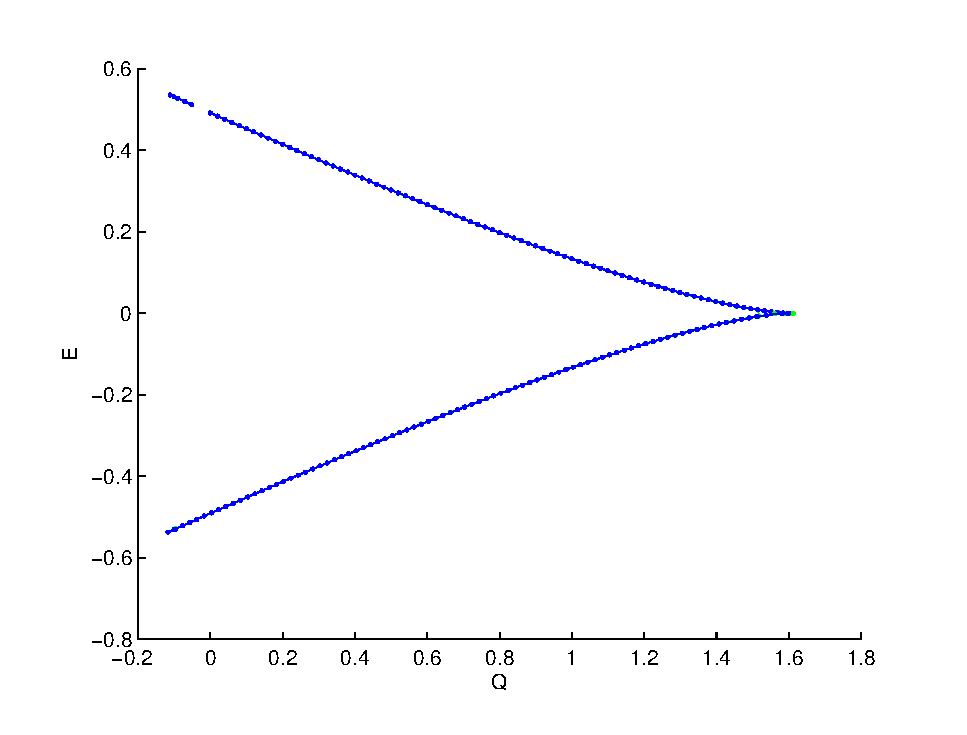
\includegraphics[scale=0.6]{images/exm3_fold_branch}\caption{Plot the fold branch. Here we see a cusp bifurcation at $(Q,E)=(1.6,0)$.\label{fig:fold_branch}}
\end{figure}
In the matlab console we have the following output:

\begin{Verbatim}[commandchars=\\\{\},fontsize=\scriptsize]
BR_CONTN warning: boundary hit.
BR_CONTN warning: boundary hit.

BR_BIFDET: Bogdanov-Takens detected near par(2) = -0.0908385124, par(4) = 0.5271860637.
Failed to correct Bogdanov-Takens point.

BR_BIFDET: Bogdanov-Takens detected near par(2) = 0.0000000000, par(4) = 0.4913668450.
Failed to correct Bogdanov-Takens point.

BR_BIFDET: Bogdanov-Takens detected near par(2) = 0.0199989457, par(4) = 0.4835320970.
Failed to correct Bogdanov-Takens point.

BR_BIFDET: Bogdanov-Takens detected near par(2) = 0.0399981183, par(4) = 0.4757164567.
Failed to correct Bogdanov-Takens point.

BR_BIFDET: Cusp detected near par(2) = 1.3179630819, par(4) = 0.0462438690.
Failed to correct cusp.

BR_BIFDET: Bogdanov-Takens detected near par(2) = 1.3179630819, par(4) = 0.0462438690.
BR_BIFDET: a = -0.2307473313, b = -0.9154839442, par(2) = 1.3000000000, par(4) = 0.0505079212.

BR_BIFDET: Cusp detected near par(2) = 1.5990696079, par(4) = -0.0000094571.
BR_BIFDET: Cusp located at  par(2) = 1.6000000000, par(4) = -0.0000000000.
BR_BIFDET: Normal form coefficients: b = -0.0000000002, c = 0.5555557861.

BR_BIFDET: Bogdanov-Takens detected near par(2) = 1.5811766051, par(4) = -0.0008560336.
Failed to correct Bogdanov-Takens point.

BR_BIFDET: Cusp detected near par(2) = 1.2852191807, par(4) = -0.0540913384.
Failed to correct cusp.

BR_BIFDET: Bogdanov-Takens detected near par(2) = 1.2852191807, par(4) = -0.0540913384.
BR_BIFDET: a = 0.2353902067, b = 0.9123599189, par(2) = 1.3000000000, par(4) = -0.0505079212. 
\end{Verbatim}

In Figure \ref{fig:fold_br_testfunctions} we have plotted the test
functions. The detection of a cusp point near a Bogdanov-Takens point
can be explained. Indeed, the test function for the Bogdanov-Takens
point $\psi_{BT}^{f}=p^{T}\Delta'(0)q$ is normalized to 1 in the
calculation for the critical normal form of the fold point. This is
done by scaling the vector $p$. Near a Bogdanov-Takens point $p^{T}\Delta'(0)q$
becomes really small, which means the length of $p$ becomes very
large in order to achieve the normalization $p^{T}\Delta'(0)q$=1
. As a result the length of the critical normal form coefficient $b$
in (\ref{eq:normal_form_fold_coef}) of a fold point becomes very
large.

\begin{figure}[h]
\begin{centering}
\includegraphics[width=1\textwidth]{images/exm3_fold_testfunctions_big}\\

\par\end{centering}

\centering{}\includegraphics[width=1\textwidth]{images/exm3_fold_testfunctions_small}\caption{Plot of test functions for fold\_br\label{fig:fold_br_testfunctions}}
\end{figure}


\clearpage

\bibliographystyle{apalike}
\bibliography{nmfm_extension_description}

\end{document}
